\documentclass[10pt,a4paper,twocolumn]{article}

% ── Page ────────────────────────────────────────────────────
\usepackage[a4paper, left=1.7cm, right=1.7cm, top=2.3cm, bottom=2.0cm,
            headheight=18pt, headsep=10pt, columnsep=6mm]{geometry}

% ── Fonts: Times-like text and maths, as in most journals ───
\usepackage[T1]{fontenc}
\usepackage[utf8]{inputenc}
\usepackage{newtxtext}
\usepackage{newtxmath}
\usepackage{microtype}

% ── Content ─────────────────────────────────────────────────
\usepackage{amsmath}
\usepackage{graphicx}
\usepackage[dvipsnames]{xcolor}
\usepackage{booktabs}
\usepackage{array}
\usepackage{tabularx}
\usepackage{enumitem}
\usepackage{listings}
\usepackage{textcomp}
\usepackage[round]{natbib}
\usepackage[font=small, labelfont=bf, labelsep=period, skip=4pt]{caption}
\usepackage{titlesec}
\usepackage{fancyhdr}
\usepackage{lastpage}
\usepackage[colorlinks=true, linkcolor=MidnightBlue, citecolor=MidnightBlue,
            urlcolor=MidnightBlue, bookmarks=true]{hyperref}

\usepackage{xurl}                          % long URLs break across lines
\usepackage{orcidlink}

% ── Journal-style headings: numbered, serif, restrained ─────
\titleformat{\section}{\normalfont\large\bfseries}{\thesection}{0.6em}{}
\titleformat{\subsection}{\normalfont\normalsize\bfseries}{\thesubsection}{0.5em}{}
\titleformat{\subsubsection}{\normalfont\normalsize\itshape}{\thesubsubsection}{0.5em}{}
\titlespacing*{\section}{0pt}{1.4ex plus 0.6ex}{0.7ex}
\titlespacing*{\subsection}{0pt}{1.1ex plus 0.4ex}{0.5ex}
\setlength{\parindent}{1em}
\setlength{\parskip}{0pt}
\raggedbottom                               % no stretched gaps to fill columns
\setlist{leftmargin=*, itemsep=0.2em, topsep=0.3em}


% ── Journal draft: plain pages, no running header ──────────
\pagestyle{plain}
\hypersetup{pdftitle={When do flood susceptibility models beat the flood record? Evidence from radar-observed floods in Bangladesh},
            pdfauthor={Md Rakib Hasan}}
\graphicspath{{../}}
% Let full-width figures and tables sit near their text in two columns.
\renewcommand{\dbltopfraction}{0.9}
\renewcommand{\dblfloatpagefraction}{0.6}
\setcounter{dbltopnumber}{3}
\renewcommand{\topfraction}{0.9}
\renewcommand{\floatpagefraction}{0.6}
% Marks work still to be done before submission. Remove every one.
\newcommand{\pending}[1]{\textcolor{red}{[PENDING: #1]}}

% ── Code listings fit a single column ──────────────────────
\lstset{basicstyle=\footnotesize\ttfamily, breaklines=true,
        columns=fullflexible, frame=tb, framerule=0.3pt,
        aboveskip=0.5em, belowskip=0.5em}

% ── Monospace that breaks at underscores ───────────────────
\makeatletter
\let\orig@texttt\texttt
\renewcommand{\texttt}[1]{%
  \ifmmode\text{\orig@texttt{#1}}\else
  \begingroup\ttfamily\def\_{\textunderscore\allowbreak}#1\endgroup\fi}
\makeatother
\newcommand{\fileref}[1]{\texttt{#1}}

% Generated by docs/build_numbers.py — do not edit by hand.
% Built 2026-10-22T18:03:17+00:00
%
% Any figure the pipeline did not produce renders as \todo{missing},
% so a gap is visible in the PDF rather than filled from memory.
\providecommand{\todo}[1]{\textbf{[TODO: #1]}}

% ---- rangpur_rajshahi ----
\newcommand{\RRAssets}{23,016}
\newcommand{\RRMappedCellShare}{12.5}
\newcommand{\RRLabelRate}{6.7}
\newcommand{\RRValAUC}{0.884}
\newcommand{\RRValAP}{0.234}
\newcommand{\RRValAPLift}{7.0}
\newcommand{\RRValBrier}{0.069}
\newcommand{\RRValBrierCalibrated}{0.029}
\newcommand{\RRValBrierBaseRate}{0.032}
\newcommand{\RRNCalibration}{1,474}
\newcommand{\RRNTrain}{18,687}
\newcommand{\RRNVal}{2,855}
\newcommand{\RRScoreMean}{0.068}
\newcommand{\RRScoreMedian}{0.013}
\newcommand{\RRKrigingVar}{0.037}
\newcommand{\RRKrigingSillRatio}{0.442}
\newcommand{\RRVariogramRange}{1.087}
\newcommand{\RRVariogramRangeKm}{115}
\newcommand{\RRNuggetSillRatio}{0.307}
\newcommand{\RRProcessed}{2026-09-29}
\newcommand{\RRNVulnComponents}{4}
\newcommand{\RRObsEvents}{5}
\newcommand{\RRObsFloodedShare}{6.7}
\newcommand{\RRObsAUC}{0.879}
\newcommand{\RRObsAPLift}{6.3}
\newcommand{\RRObsBrierCalibrated}{0.030}
\newcommand{\RRProxyPOD}{0.151}
\newcommand{\RRProxyFAR}{0.517}
\newcommand{\RRProxyCSI}{0.130}
\newcommand{\RRProxyKappa}{0.144}
\newcommand{\RRProxyShare}{6.6}
\newcommand{\RRObservedShare}{21.2}
\newcommand{\RRMinEvents}{2}
\newcommand{\RRSurfaceKrigedObsAUC}{0.666}
\newcommand{\RRSurfaceTerrainObsAUC}{0.657}
\newcommand{\RRProxyTrainedObsAUC}{0.809}
\newcommand{\RRProxyTrainedObsAPLift}{2.4}
\newcommand{\RRCalibBlockRate}{6.4}
\newcommand{\RRTestBlockRate}{3.3}
\newcommand{\RRKrigedGridSD}{0.127}
\newcommand{\RRTerrainGridSD}{0.238}
\newcommand{\RRHazardAUC}{0.621}
\newcommand{\RRHazardAP}{0.080}
\newcommand{\RRHazCoefElevation}{\ensuremath{-}0.811}
\newcommand{\RRHazCoefSlope}{0.027}
\newcommand{\RRHazCoefTwi}{0.064}
\newcommand{\RRHazCoefHand}{\ensuremath{-}0.032}
\newcommand{\RRHazCoefFlowAcc}{\ensuremath{-}0.021}
\newcommand{\RRBenchGraphAUC}{0.789}
\newcommand{\RRBenchGraphSD}{0.047}
\newcommand{\RRBenchGraphLift}{3.6}
\newcommand{\RRBenchLogisticAUC}{0.786}
\newcommand{\RRBenchLogisticSD}{0.039}
\newcommand{\RRBenchLogisticLift}{3.3}
\newcommand{\RRBenchForestAUC}{0.816}
\newcommand{\RRBenchForestSD}{0.044}
\newcommand{\RRBenchForestLift}{4.7}
\newcommand{\RRBenchBoostingAUC}{0.817}
\newcommand{\RRBenchBoostingSD}{0.045}
\newcommand{\RRBenchBoostingLift}{4.2}
\newcommand{\RRBenchTwiAUC}{0.517}
\newcommand{\RRBenchTwiSD}{0.030}
\newcommand{\RRBenchTwiLift}{1.2}
\newcommand{\RRBenchBest}{gradient boosting}
\newcommand{\RRBenchDiff}{\ensuremath{-}0.028}
\newcommand{\RRBenchGap}{0.028}
\newcommand{\RRBenchDiffP}{=0.003}
\newcommand{\RRBenchAhead}{2}
\newcommand{\RRBenchSeeds}{20}
\newcommand{\RRLabelObsAUC}{0.817}
\newcommand{\RRLabelObsSD}{0.045}
\newcommand{\RRLabelProxyAUC}{0.716}
\newcommand{\RRLabelProxySD}{0.055}
\newcommand{\RRLabelGap}{0.101}
\newcommand{\RRLabelGapP}{<0.001}
\newcommand{\RRLabelAhead}{20}
\newcommand{\RRTempAUC}{0.801}
\newcommand{\RRTempSD}{0.063}
\newcommand{\RRTempLift}{6.4}
\newcommand{\RRTempAllAUC}{0.794}
\newcommand{\RRTempPastAUC}{0.896}
\newcommand{\RRTempPastSD}{0.042}
\newcommand{\RRTempPastLift}{21.7}
\newcommand{\RRTempMinusPast}{\ensuremath{-}0.094}
\newcommand{\RRTempMinusPastP}{=0.009}
\newcommand{\RRTempAheadPast}{2}
\newcommand{\RRTempMinusAll}{0.008}
\newcommand{\RRTempMinusAllP}{=0.281}
\newcommand{\RRTempPastGap}{0.094}
\newcommand{\RRTempAllGap}{0.008}
\newcommand{\RRTempSeeds}{20}
\newcommand{\RRTempTestRate}{2.8}
\newcommand{\RRTempProxyAUC}{0.732}
\newcommand{\RRTempProxySD}{0.067}
\newcommand{\RRTempProxyGap}{0.069}
\newcommand{\RRTempProxyGapP}{=0.013}
\newcommand{\RRTempProxyAhead}{18}
\newcommand{\RRXcCells}{645,527}
\newcommand{\RRXcSOneShare}{19.7}
\newcommand{\RRXcGfdShare}{13.2}
\newcommand{\RRXcPOD}{0.559}
\newcommand{\RRXcFAR}{0.624}
\newcommand{\RRXcCSI}{0.290}
\newcommand{\RRXcKappa}{0.346}
\newcommand{\RRXcAgree}{81.9}
\newcommand{\RRXcAUC}{0.783}
\newcommand{\RRImpElevation}{0.086}
\newcommand{\RRImpOtherTerrainMax}{0.000}
\newcommand{\RRImpTerrain}{0.080}
\newcommand{\RRImpAccess}{0.110}
\newcommand{\RRImpPopulation}{0.081}
\newcommand{\RRImpAssetType}{0.043}
\newcommand{\RRPersistAlwaysAssetShare}{97.1}
\newcommand{\RRPersistAlwaysPosShare}{42.1}
\newcommand{\RRPersistAlwaysModelAUC}{0.752}
\newcommand{\RRPersistAlwaysRecordAUC}{0.815}
\newcommand{\RRPersistAlwaysGap}{0.063}
\newcommand{\RRPersistAlwaysP}{=0.130}
\newcommand{\RRPersistAlwaysAhead}{6}
\newcommand{\RRPersistAlwaysRecordAhead}{14}
\newcommand{\RRPersistWaterAssetShare}{93.7}
\newcommand{\RRPersistWaterPosShare}{63.8}
\newcommand{\RRPersistWaterModelAUC}{0.762}
\newcommand{\RRPersistWaterRecordAUC}{0.833}
\newcommand{\RRPersistWaterGap}{0.071}
\newcommand{\RRPersistWaterP}{=0.146}
\newcommand{\RRPersistWaterAhead}{5}
\newcommand{\RRPersistWaterRecordAhead}{15}
\newcommand{\RRBlockTenSpatialAUC}{0.817}
\newcommand{\RRBlockTenSeeds}{20}
\newcommand{\RRBlockTenModelAUC}{0.801}
\newcommand{\RRBlockTenRecordAUC}{0.896}
\newcommand{\RRBlockTenTempGap}{0.094}
\newcommand{\RRBlockTenTempP}{=0.009}
\newcommand{\RRBlockTenTempAhead}{2}
\newcommand{\RRBlockTenTempSeeds}{20}
\newcommand{\RRBlockTwentySpatialAUC}{0.792}
\newcommand{\RRBlockTwentySeeds}{20}
\newcommand{\RRBlockTwentyModelAUC}{0.754}
\newcommand{\RRBlockTwentyRecordAUC}{0.884}
\newcommand{\RRBlockTwentyTempGap}{0.130}
\newcommand{\RRBlockTwentyTempP}{<0.001}
\newcommand{\RRBlockTwentyTempAhead}{0}
\newcommand{\RRBlockTwentyTempSeeds}{20}
\newcommand{\RRBlockFortySpatialAUC}{0.791}
\newcommand{\RRBlockFortySeeds}{20}
\newcommand{\RRBlockFortyModelAUC}{0.750}
\newcommand{\RRBlockFortyRecordAUC}{0.876}
\newcommand{\RRBlockFortyTempGap}{0.126}
\newcommand{\RRBlockFortyTempP}{=0.004}
\newcommand{\RRBlockFortyTempAhead}{1}
\newcommand{\RRBlockFortyTempSeeds}{20}
\newcommand{\RRTargetAnyAUC}{0.763}
\newcommand{\RRTargetAnyGap}{0.133}
\newcommand{\RRTargetAnyP}{<0.001}
\newcommand{\RRTargetAnyAhead}{0}
\newcommand{\RRTargetFracAUC}{0.765}
\newcommand{\RRTargetFracGap}{0.131}
\newcommand{\RRTargetFracP}{=0.003}
\newcommand{\RRTargetFracAhead}{1}
\newcommand{\RRSingleSatModelAUC}{0.795}
\newcommand{\RRSingleSatRecordAUC}{0.891}
\newcommand{\RRSingleSatGap}{0.097}
\newcommand{\RRSingleSatP}{=0.005}
\newcommand{\RREarlyExtentMin}{19.9}
\newcommand{\RREarlyExtentMax}{24.8}
\newcommand{\RRLateExtentMin}{4.9}
\newcommand{\RRLateExtentMax}{8.3}
\newcommand{\RRSingleSatShrinkMax}{15.7}
\newcommand{\RRDefaultSeedRank}{2}
\newcommand{\RRHazardHeldoutAUC}{0.656}
\newcommand{\RRHazardHeldoutSD}{0.039}
\newcommand{\RRPastFeatAUC}{0.924}
\newcommand{\RRPastFeatSD}{0.035}
\newcommand{\RRPastFeatWithoutAUC}{0.790}
\newcommand{\RRPastFeatOnlyAUC}{0.896}
\newcommand{\RRPastFeatOverPast}{0.029}
\newcommand{\RRPastFeatOverPastP}{=0.020}
\newcommand{\RRPastFeatOverPastAhead}{16}
\newcommand{\RRPastFeatOverWithout}{0.134}
\newcommand{\RRPastFeatOverWithoutP}{<0.001}
\newcommand{\RRPastFeatUnseenAUC}{0.729}
\newcommand{\RRPastFeatUnseenShare}{87.7}
\newcommand{\RRPastFeatUnseenPos}{16.9}
\newcommand{\RRSkillModel}{\ensuremath{-}0.905}
\newcommand{\RRSkillPastFeat}{0.276}
\newcommand{\RRRecordLenOneRec}{0.812}
\newcommand{\RRRecordLenOneModel}{0.768}
\newcommand{\RRRecordLenTwoRec}{0.873}
\newcommand{\RRRecordLenTwoModel}{0.788}
\newcommand{\RRRecordLenThreeRec}{0.896}
\newcommand{\RRRecordLenThreeModel}{0.801}
\newcommand{\RRPlanListShare}{15.5}
\newcommand{\RROofModelAUC}{0.857}
\newcommand{\RROofRecordAUC}{0.942}
\newcommand{\RROofBothAUC}{0.950}
\newcommand{\RROofGapLow}{\ensuremath{-}0.127}
\newcommand{\RROofGapHigh}{\ensuremath{-}0.064}
\newcommand{\RROofBothGapLow}{\ensuremath{-}0.003}
\newcommand{\RROofBothGapHigh}{0.042}
\newcommand{\RRListFiveRec}{71.9}
\newcommand{\RRListFiveModel}{41.8}
\newcommand{\RRListFiveBoth}{64.3}
\newcommand{\RRListTenRec}{87.1}
\newcommand{\RRListTenModel}{59.8}
\newcommand{\RRListTenBoth}{85.2}
\newcommand{\RRListTwentyRec}{93.8}
\newcommand{\RRListTwentyModel}{71.6}
\newcommand{\RRListTwentyBoth}{94.7}
\newcommand{\RRListThirtyRec}{94.6}
\newcommand{\RRListThirtyModel}{76.7}
\newcommand{\RRListThirtyBoth}{96.3}
\newcommand{\RRPlanAllFlooded}{644}
\newcommand{\RRPlanAllRecord}{93.2}
\newcommand{\RRPlanAllModel}{68.5}
\newcommand{\RRPlanAllBoth}{93.2}
\newcommand{\RRPlanAllModelOnly}{17}
\newcommand{\RRPlanAllRecordOnly}{176}
\newcommand{\RRPlanFacilFlooded}{11}
\newcommand{\RRPlanFacilRecord}{36.4}
\newcommand{\RRPlanFacilModel}{18.2}
\newcommand{\RRPlanFacilBoth}{45.5}
\newcommand{\RRPlanFacilModelOnly}{2}
\newcommand{\RRPlanFacilRecordOnly}{4}
\newcommand{\RRPlanTransFlooded}{162}
\newcommand{\RRPlanTransRecord}{88.3}
\newcommand{\RRPlanTransModel}{34.0}
\newcommand{\RRPlanTransBoth}{88.3}
\newcommand{\RRPlanTransModelOnly}{4}
\newcommand{\RRPlanTransRecordOnly}{92}
\newcommand{\RRSensEqualTypesRho}{0.942}
\newcommand{\RRSensPopOnlyRho}{0.663}
\newcommand{\RRSensExposureDoubleRho}{0.946}
\newcommand{\RRSensExposureDoubleTop}{0.829}
\newcommand{\RRSensRandomRho}{0.963}
\newcommand{\RRSensRandomRhoMin}{0.914}
\newcommand{\RRSensRandomTop}{0.870}
\newcommand{\RRSensDraws}{20}
\newcommand{\RRNUnions}{1,339}
\newcommand{\RRNUnionsScored}{1,199}
\newcommand{\RRNUpazilas}{148}
\newcommand{\RRNUpazilasScored}{147}
\newcommand{\RRNDistricts}{21}
\newcommand{\RRNDistrictsScored}{21}

% ---- sylhet ----
\newcommand{\SylhetAssets}{13,374}
\newcommand{\SylhetMappedCellShare}{10.3}
\newcommand{\SylhetLabelRate}{14.7}
\newcommand{\SylhetValAUC}{0.934}
\newcommand{\SylhetValAP}{0.639}
\newcommand{\SylhetValAPLift}{6.1}
\newcommand{\SylhetValBrier}{0.073}
\newcommand{\SylhetValBrierCalibrated}{0.057}
\newcommand{\SylhetValBrierBaseRate}{0.094}
\newcommand{\SylhetNCalibration}{953}
\newcommand{\SylhetNTrain}{11,026}
\newcommand{\SylhetNVal}{1,395}
\newcommand{\SylhetScoreMean}{0.274}
\newcommand{\SylhetScoreMedian}{0.079}
\newcommand{\SylhetKrigingVar}{0.095}
\newcommand{\SylhetKrigingSillRatio}{0.933}
\newcommand{\SylhetVariogramRange}{0.136}
\newcommand{\SylhetVariogramRangeKm}{14}
\newcommand{\SylhetNuggetSillRatio}{0.742}
\newcommand{\SylhetProcessed}{2026-09-29}
\newcommand{\SylhetNVulnComponents}{4}
\newcommand{\SylhetObsEvents}{4}
\newcommand{\SylhetObsFloodedShare}{14.7}
\newcommand{\SylhetObsAUC}{0.934}
\newcommand{\SylhetObsAPLift}{6.0}
\newcommand{\SylhetObsBrierCalibrated}{0.057}
\newcommand{\SylhetProxyPOD}{0.273}
\newcommand{\SylhetProxyFAR}{0.626}
\newcommand{\SylhetProxyCSI}{0.187}
\newcommand{\SylhetProxyKappa}{0.176}
\newcommand{\SylhetProxyShare}{14.7}
\newcommand{\SylhetObservedShare}{20.1}
\newcommand{\SylhetMinEvents}{2}
\newcommand{\SylhetSurfaceKrigedObsAUC}{0.544}
\newcommand{\SylhetSurfaceTerrainObsAUC}{0.822}
\newcommand{\SylhetProxyTrainedObsAUC}{0.847}
\newcommand{\SylhetProxyTrainedObsAPLift}{3.3}
\newcommand{\SylhetCalibBlockRate}{13.7}
\newcommand{\SylhetTestBlockRate}{10.5}
\newcommand{\SylhetKrigedGridSD}{0.108}
\newcommand{\SylhetTerrainGridSD}{0.262}
\newcommand{\SylhetHazardAUC}{0.788}
\newcommand{\SylhetHazardAP}{0.263}
\newcommand{\SylhetHazCoefElevation}{\ensuremath{-}1.264}
\newcommand{\SylhetHazCoefSlope}{\ensuremath{-}0.244}
\newcommand{\SylhetHazCoefTwi}{\ensuremath{-}0.102}
\newcommand{\SylhetHazCoefHand}{0.033}
\newcommand{\SylhetHazCoefFlowAcc}{\ensuremath{-}0.227}
\newcommand{\SylhetBenchGraphAUC}{0.854}
\newcommand{\SylhetBenchGraphSD}{0.039}
\newcommand{\SylhetBenchGraphLift}{3.8}
\newcommand{\SylhetBenchLogisticAUC}{0.855}
\newcommand{\SylhetBenchLogisticSD}{0.036}
\newcommand{\SylhetBenchLogisticLift}{3.4}
\newcommand{\SylhetBenchForestAUC}{0.845}
\newcommand{\SylhetBenchForestSD}{0.052}
\newcommand{\SylhetBenchForestLift}{3.8}
\newcommand{\SylhetBenchBoostingAUC}{0.857}
\newcommand{\SylhetBenchBoostingSD}{0.042}
\newcommand{\SylhetBenchBoostingLift}{3.9}
\newcommand{\SylhetBenchTwiAUC}{0.535}
\newcommand{\SylhetBenchTwiSD}{0.029}
\newcommand{\SylhetBenchTwiLift}{1.1}
\newcommand{\SylhetBenchBest}{gradient boosting}
\newcommand{\SylhetBenchDiff}{\ensuremath{-}0.003}
\newcommand{\SylhetBenchGap}{0.003}
\newcommand{\SylhetBenchDiffP}{=0.832}
\newcommand{\SylhetBenchAhead}{7}
\newcommand{\SylhetBenchSeeds}{20}
\newcommand{\SylhetLabelObsAUC}{0.857}
\newcommand{\SylhetLabelObsSD}{0.042}
\newcommand{\SylhetLabelProxyAUC}{0.770}
\newcommand{\SylhetLabelProxySD}{0.048}
\newcommand{\SylhetLabelGap}{0.087}
\newcommand{\SylhetLabelGapP}{=0.003}
\newcommand{\SylhetLabelAhead}{19}
\newcommand{\SylhetTempAUC}{0.797}
\newcommand{\SylhetTempSD}{0.064}
\newcommand{\SylhetTempLift}{3.0}
\newcommand{\SylhetTempAllAUC}{0.850}
\newcommand{\SylhetTempPastAUC}{0.851}
\newcommand{\SylhetTempPastSD}{0.039}
\newcommand{\SylhetTempPastLift}{3.8}
\newcommand{\SylhetTempMinusPast}{\ensuremath{-}0.054}
\newcommand{\SylhetTempMinusPastP}{=0.036}
\newcommand{\SylhetTempAheadPast}{4}
\newcommand{\SylhetTempMinusAll}{\ensuremath{-}0.053}
\newcommand{\SylhetTempMinusAllP}{=0.020}
\newcommand{\SylhetTempPastGap}{0.054}
\newcommand{\SylhetTempAllGap}{0.053}
\newcommand{\SylhetTempSeeds}{20}
\newcommand{\SylhetTempTestRate}{17.7}
\newcommand{\SylhetTempProxyAUC}{0.773}
\newcommand{\SylhetTempProxySD}{0.043}
\newcommand{\SylhetTempProxyGap}{0.024}
\newcommand{\SylhetTempProxyGapP}{=0.333}
\newcommand{\SylhetTempProxyAhead}{15}
\newcommand{\SylhetXcCells}{342,128}
\newcommand{\SylhetXcSOneShare}{13.2}
\newcommand{\SylhetXcGfdShare}{23.3}
\newcommand{\SylhetXcPOD}{0.396}
\newcommand{\SylhetXcFAR}{0.300}
\newcommand{\SylhetXcCSI}{0.339}
\newcommand{\SylhetXcKappa}{0.406}
\newcommand{\SylhetXcAgree}{82.0}
\newcommand{\SylhetXcAUC}{0.746}
\newcommand{\SylhetImpElevation}{0.220}
\newcommand{\SylhetImpOtherTerrainMax}{0.009}
\newcommand{\SylhetImpTerrain}{0.214}
\newcommand{\SylhetImpAccess}{0.133}
\newcommand{\SylhetImpPopulation}{0.032}
\newcommand{\SylhetImpAssetType}{0.020}
\newcommand{\SylhetPersistAlwaysAssetShare}{95.4}
\newcommand{\SylhetPersistAlwaysPosShare}{76.1}
\newcommand{\SylhetPersistAlwaysModelAUC}{0.774}
\newcommand{\SylhetPersistAlwaysRecordAUC}{0.815}
\newcommand{\SylhetPersistAlwaysGap}{0.040}
\newcommand{\SylhetPersistAlwaysP}{=0.185}
\newcommand{\SylhetPersistAlwaysAhead}{8}
\newcommand{\SylhetPersistAlwaysRecordAhead}{12}
\newcommand{\SylhetPersistWaterAssetShare}{72.0}
\newcommand{\SylhetPersistWaterPosShare}{29.9}
\newcommand{\SylhetPersistWaterModelAUC}{0.799}
\newcommand{\SylhetPersistWaterRecordAUC}{0.794}
\newcommand{\SylhetPersistWaterGap}{0.005}
\newcommand{\SylhetPersistWaterP}{=0.912}
\newcommand{\SylhetPersistWaterAhead}{12}
\newcommand{\SylhetPersistWaterRecordAhead}{8}
\newcommand{\SylhetBlockTenSpatialAUC}{0.857}
\newcommand{\SylhetBlockTenSeeds}{20}
\newcommand{\SylhetBlockTenModelAUC}{0.797}
\newcommand{\SylhetBlockTenRecordAUC}{0.851}
\newcommand{\SylhetBlockTenTempGap}{0.054}
\newcommand{\SylhetBlockTenTempP}{=0.036}
\newcommand{\SylhetBlockTenTempAhead}{4}
\newcommand{\SylhetBlockTenTempSeeds}{20}
\newcommand{\SylhetBlockTwentySpatialAUC}{0.856}
\newcommand{\SylhetBlockTwentySeeds}{20}
\newcommand{\SylhetBlockTwentyModelAUC}{0.795}
\newcommand{\SylhetBlockTwentyRecordAUC}{0.850}
\newcommand{\SylhetBlockTwentyTempGap}{0.054}
\newcommand{\SylhetBlockTwentyTempP}{=0.028}
\newcommand{\SylhetBlockTwentyTempAhead}{3}
\newcommand{\SylhetBlockTwentyTempSeeds}{20}
\newcommand{\SylhetBlockFortySpatialAUC}{0.836}
\newcommand{\SylhetBlockFortySeeds}{15}
\newcommand{\SylhetBlockFortyModelAUC}{0.774}
\newcommand{\SylhetBlockFortyRecordAUC}{0.847}
\newcommand{\SylhetBlockFortyTempGap}{0.073}
\newcommand{\SylhetBlockFortyTempP}{=0.017}
\newcommand{\SylhetBlockFortyTempAhead}{1}
\newcommand{\SylhetBlockFortyTempSeeds}{15}
\newcommand{\SylhetTargetAnyAUC}{0.834}
\newcommand{\SylhetTargetAnyGap}{0.017}
\newcommand{\SylhetTargetAnyP}{=0.441}
\newcommand{\SylhetTargetAnyAhead}{7}
\newcommand{\SylhetTargetFracAUC}{0.835}
\newcommand{\SylhetTargetFracGap}{0.016}
\newcommand{\SylhetTargetFracP}{=0.401}
\newcommand{\SylhetTargetFracAhead}{7}
\newcommand{\SylhetSingleSatModelAUC}{0.797}
\newcommand{\SylhetSingleSatRecordAUC}{0.851}
\newcommand{\SylhetSingleSatGap}{0.054}
\newcommand{\SylhetSingleSatP}{=0.036}
\newcommand{\SylhetEarlyExtentMin}{13.3}
\newcommand{\SylhetEarlyExtentMax}{34.1}
\newcommand{\SylhetLateExtentMin}{20.4}
\newcommand{\SylhetLateExtentMax}{31.2}
\newcommand{\SylhetSingleSatShrinkMax}{0.0}
\newcommand{\SylhetDefaultSeedRank}{1}
\newcommand{\SylhetHazardHeldoutAUC}{0.763}
\newcommand{\SylhetHazardHeldoutSD}{0.036}
\newcommand{\SylhetPastFeatAUC}{0.849}
\newcommand{\SylhetPastFeatSD}{0.046}
\newcommand{\SylhetPastFeatWithoutAUC}{0.837}
\newcommand{\SylhetPastFeatOnlyAUC}{0.851}
\newcommand{\SylhetPastFeatOverPast}{\ensuremath{-}0.002}
\newcommand{\SylhetPastFeatOverPastP}{=0.881}
\newcommand{\SylhetPastFeatOverPastAhead}{9}
\newcommand{\SylhetPastFeatOverWithout}{0.011}
\newcommand{\SylhetPastFeatOverWithoutP}{=0.196}
\newcommand{\SylhetPastFeatUnseenAUC}{0.777}
\newcommand{\SylhetPastFeatUnseenShare}{79.8}
\newcommand{\SylhetPastFeatUnseenPos}{22.3}
\newcommand{\SylhetSkillModel}{\ensuremath{-}0.364}
\newcommand{\SylhetSkillPastFeat}{\ensuremath{-}0.016}
\newcommand{\SylhetRecordLenOneRec}{0.726}
\newcommand{\SylhetRecordLenOneModel}{0.794}
\newcommand{\SylhetRecordLenTwoRec}{0.851}
\newcommand{\SylhetRecordLenTwoModel}{0.797}
\newcommand{\SylhetPlanListShare}{20.8}
\newcommand{\SylhetOofModelAUC}{0.800}
\newcommand{\SylhetOofRecordAUC}{0.855}
\newcommand{\SylhetOofBothAUC}{0.865}
\newcommand{\SylhetOofGapLow}{\ensuremath{-}0.090}
\newcommand{\SylhetOofGapHigh}{\ensuremath{-}0.019}
\newcommand{\SylhetOofBothGapLow}{\ensuremath{-}0.015}
\newcommand{\SylhetOofBothGapHigh}{0.032}
\newcommand{\SylhetListFiveRec}{25.1}
\newcommand{\SylhetListFiveModel}{18.1}
\newcommand{\SylhetListFiveBoth}{23.3}
\newcommand{\SylhetListTenRec}{41.3}
\newcommand{\SylhetListTenModel}{30.4}
\newcommand{\SylhetListTenBoth}{37.0}
\newcommand{\SylhetListTwentyRec}{74.9}
\newcommand{\SylhetListTwentyModel}{49.4}
\newcommand{\SylhetListTwentyBoth}{60.5}
\newcommand{\SylhetListThirtyRec}{80.1}
\newcommand{\SylhetListThirtyModel}{65.0}
\newcommand{\SylhetListThirtyBoth}{74.4}
\newcommand{\SylhetPlanAllFlooded}{2,367}
\newcommand{\SylhetPlanAllRecord}{77.9}
\newcommand{\SylhetPlanAllModel}{50.6}
\newcommand{\SylhetPlanAllBoth}{62.0}
\newcommand{\SylhetPlanAllModelOnly}{168}
\newcommand{\SylhetPlanAllRecordOnly}{814}
\newcommand{\SylhetPlanFacilFlooded}{32}
\newcommand{\SylhetPlanFacilRecord}{40.6}
\newcommand{\SylhetPlanFacilModel}{3.1}
\newcommand{\SylhetPlanFacilBoth}{6.2}
\newcommand{\SylhetPlanFacilModelOnly}{1}
\newcommand{\SylhetPlanFacilRecordOnly}{13}
\newcommand{\SylhetPlanTransFlooded}{696}
\newcommand{\SylhetPlanTransRecord}{71.6}
\newcommand{\SylhetPlanTransModel}{56.8}
\newcommand{\SylhetPlanTransBoth}{32.8}
\newcommand{\SylhetPlanTransModelOnly}{87}
\newcommand{\SylhetPlanTransRecordOnly}{190}
\newcommand{\SylhetSensEqualTypesRho}{0.901}
\newcommand{\SylhetSensPopOnlyRho}{0.431}
\newcommand{\SylhetSensExposureDoubleRho}{0.952}
\newcommand{\SylhetSensExposureDoubleTop}{0.779}
\newcommand{\SylhetSensRandomRho}{0.956}
\newcommand{\SylhetSensRandomRhoMin}{0.913}
\newcommand{\SylhetSensRandomTop}{0.802}
\newcommand{\SylhetSensDraws}{20}
\newcommand{\SylhetNUnions}{717}
\newcommand{\SylhetNUnionsScored}{642}
\newcommand{\SylhetNUpazilas}{78}
\newcommand{\SylhetNUpazilasScored}{78}
\newcommand{\SylhetNDistricts}{10}
\newcommand{\SylhetNDistrictsScored}{10}

% ---- sw_coastal ----
\newcommand{\CoastalAssets}{29,545}
\newcommand{\CoastalMappedCellShare}{11.6}
\newcommand{\CoastalLabelRate}{4.5}
\newcommand{\CoastalValAUC}{0.794}
\newcommand{\CoastalValAP}{0.044}
\newcommand{\CoastalValAPLift}{2.5}
\newcommand{\CoastalValBrier}{0.134}
\newcommand{\CoastalValBrierCalibrated}{0.039}
\newcommand{\CoastalValBrierBaseRate}{0.017}
\newcommand{\CoastalNCalibration}{2,472}
\newcommand{\CoastalNTrain}{23,635}
\newcommand{\CoastalNVal}{3,438}
\newcommand{\CoastalScoreMean}{0.226}
\newcommand{\CoastalScoreMedian}{0.084}
\newcommand{\CoastalKrigingVar}{0.064}
\newcommand{\CoastalKrigingSillRatio}{0.844}
\newcommand{\CoastalVariogramRange}{0.289}
\newcommand{\CoastalVariogramRangeKm}{31}
\newcommand{\CoastalNuggetSillRatio}{0.702}
\newcommand{\CoastalProcessed}{2026-09-29}
\newcommand{\CoastalNVulnComponents}{4}
\newcommand{\CoastalObsEvents}{4}
\newcommand{\CoastalObsFloodedShare}{4.4}
\newcommand{\CoastalObsAUC}{0.786}
\newcommand{\CoastalObsAPLift}{2.4}
\newcommand{\CoastalObsBrierCalibrated}{0.039}
\newcommand{\CoastalProxyPOD}{0.224}
\newcommand{\CoastalProxyFAR}{0.956}
\newcommand{\CoastalProxyCSI}{0.039}
\newcommand{\CoastalProxyKappa}{0.037}
\newcommand{\CoastalProxyShare}{11.8}
\newcommand{\CoastalObservedShare}{2.3}
\newcommand{\CoastalMinEvents}{1}
\newcommand{\CoastalSurfaceKrigedObsAUC}{0.538}
\newcommand{\CoastalSurfaceTerrainObsAUC}{0.542}
\newcommand{\CoastalProxyTrainedObsAUC}{0.814}
\newcommand{\CoastalProxyTrainedObsAPLift}{3.4}
\newcommand{\CoastalCalibBlockRate}{5.5}
\newcommand{\CoastalTestBlockRate}{1.7}
\newcommand{\CoastalKrigedGridSD}{0.133}
\newcommand{\CoastalTerrainGridSD}{0.378}
\newcommand{\CoastalHazardAUC}{0.757}
\newcommand{\CoastalHazardAP}{0.062}
\newcommand{\CoastalHazCoefElevation}{\ensuremath{-}1.166}
\newcommand{\CoastalHazCoefSlope}{\ensuremath{-}0.590}
\newcommand{\CoastalHazCoefTwi}{\ensuremath{-}0.270}
\newcommand{\CoastalHazCoefHand}{0.107}
\newcommand{\CoastalHazCoefFlowAcc}{\ensuremath{-}0.193}
\newcommand{\CoastalBenchGraphAUC}{0.817}
\newcommand{\CoastalBenchGraphSD}{0.057}
\newcommand{\CoastalBenchGraphLift}{4.1}
\newcommand{\CoastalBenchLogisticAUC}{0.809}
\newcommand{\CoastalBenchLogisticSD}{0.046}
\newcommand{\CoastalBenchLogisticLift}{3.1}
\newcommand{\CoastalBenchForestAUC}{0.838}
\newcommand{\CoastalBenchForestSD}{0.049}
\newcommand{\CoastalBenchForestLift}{5.0}
\newcommand{\CoastalBenchBoostingAUC}{0.839}
\newcommand{\CoastalBenchBoostingSD}{0.046}
\newcommand{\CoastalBenchBoostingLift}{4.5}
\newcommand{\CoastalBenchTwiAUC}{0.577}
\newcommand{\CoastalBenchTwiSD}{0.041}
\newcommand{\CoastalBenchTwiLift}{1.3}
\newcommand{\CoastalBenchBest}{gradient boosting}
\newcommand{\CoastalBenchDiff}{\ensuremath{-}0.022}
\newcommand{\CoastalBenchGap}{0.022}
\newcommand{\CoastalBenchDiffP}{=0.243}
\newcommand{\CoastalBenchAhead}{6}
\newcommand{\CoastalBenchSeeds}{20}
\newcommand{\CoastalLabelObsAUC}{0.839}
\newcommand{\CoastalLabelObsSD}{0.046}
\newcommand{\CoastalLabelProxyAUC}{0.758}
\newcommand{\CoastalLabelProxySD}{0.053}
\newcommand{\CoastalLabelGap}{0.080}
\newcommand{\CoastalLabelGapP}{<0.001}
\newcommand{\CoastalLabelAhead}{19}
\newcommand{\CoastalTempAUC}{0.807}
\newcommand{\CoastalTempSD}{0.055}
\newcommand{\CoastalTempLift}{5.3}
\newcommand{\CoastalTempAllAUC}{0.834}
\newcommand{\CoastalTempPastAUC}{0.668}
\newcommand{\CoastalTempPastSD}{0.072}
\newcommand{\CoastalTempPastLift}{10.9}
\newcommand{\CoastalTempMinusPast}{0.138}
\newcommand{\CoastalTempMinusPastP}{<0.001}
\newcommand{\CoastalTempAheadPast}{19}
\newcommand{\CoastalTempMinusAll}{\ensuremath{-}0.028}
\newcommand{\CoastalTempMinusAllP}{=0.052}
\newcommand{\CoastalTempPastGap}{0.138}
\newcommand{\CoastalTempAllGap}{0.028}
\newcommand{\CoastalTempSeeds}{20}
\newcommand{\CoastalTempTestRate}{2.9}
\newcommand{\CoastalTempProxyAUC}{0.736}
\newcommand{\CoastalTempProxySD}{0.066}
\newcommand{\CoastalTempProxyGap}{0.071}
\newcommand{\CoastalTempProxyGapP}{=0.004}
\newcommand{\CoastalTempProxyAhead}{18}
\newcommand{\CoastalXcCells}{\todo{missing}}
\newcommand{\CoastalXcSOneShare}{\todo{missing}}
\newcommand{\CoastalXcGfdShare}{\todo{missing}}
\newcommand{\CoastalXcPOD}{\todo{missing}}
\newcommand{\CoastalXcFAR}{\todo{missing}}
\newcommand{\CoastalXcCSI}{\todo{missing}}
\newcommand{\CoastalXcKappa}{\todo{missing}}
\newcommand{\CoastalXcAgree}{\todo{missing}}
\newcommand{\CoastalXcAUC}{\todo{missing}}
\newcommand{\CoastalImpElevation}{0.129}
\newcommand{\CoastalImpOtherTerrainMax}{0.007}
\newcommand{\CoastalImpTerrain}{0.132}
\newcommand{\CoastalImpAccess}{0.142}
\newcommand{\CoastalImpPopulation}{0.050}
\newcommand{\CoastalImpAssetType}{0.020}
\newcommand{\CoastalPersistAlwaysAssetShare}{99.9}
\newcommand{\CoastalPersistAlwaysPosShare}{98.4}
\newcommand{\CoastalPersistAlwaysModelAUC}{0.806}
\newcommand{\CoastalPersistAlwaysRecordAUC}{0.667}
\newcommand{\CoastalPersistAlwaysGap}{0.140}
\newcommand{\CoastalPersistAlwaysP}{<0.001}
\newcommand{\CoastalPersistAlwaysAhead}{19}
\newcommand{\CoastalPersistAlwaysRecordAhead}{1}
\newcommand{\CoastalPersistWaterAssetShare}{78.1}
\newcommand{\CoastalPersistWaterPosShare}{50.1}
\newcommand{\CoastalPersistWaterModelAUC}{0.827}
\newcommand{\CoastalPersistWaterRecordAUC}{0.661}
\newcommand{\CoastalPersistWaterGap}{0.166}
\newcommand{\CoastalPersistWaterP}{<0.001}
\newcommand{\CoastalPersistWaterAhead}{20}
\newcommand{\CoastalPersistWaterRecordAhead}{0}
\newcommand{\CoastalBlockTenSpatialAUC}{0.839}
\newcommand{\CoastalBlockTenSeeds}{20}
\newcommand{\CoastalBlockTenModelAUC}{0.807}
\newcommand{\CoastalBlockTenRecordAUC}{0.668}
\newcommand{\CoastalBlockTenTempGap}{0.138}
\newcommand{\CoastalBlockTenTempP}{<0.001}
\newcommand{\CoastalBlockTenTempAhead}{19}
\newcommand{\CoastalBlockTenTempSeeds}{20}
\newcommand{\CoastalBlockTwentySpatialAUC}{0.796}
\newcommand{\CoastalBlockTwentySeeds}{20}
\newcommand{\CoastalBlockTwentyModelAUC}{0.738}
\newcommand{\CoastalBlockTwentyRecordAUC}{0.660}
\newcommand{\CoastalBlockTwentyTempGap}{0.079}
\newcommand{\CoastalBlockTwentyTempP}{=0.182}
\newcommand{\CoastalBlockTwentyTempAhead}{14}
\newcommand{\CoastalBlockTwentyTempSeeds}{20}
\newcommand{\CoastalBlockFortySpatialAUC}{0.774}
\newcommand{\CoastalBlockFortySeeds}{19}
\newcommand{\CoastalBlockFortyModelAUC}{0.729}
\newcommand{\CoastalBlockFortyRecordAUC}{0.676}
\newcommand{\CoastalBlockFortyTempGap}{0.053}
\newcommand{\CoastalBlockFortyTempP}{=0.423}
\newcommand{\CoastalBlockFortyTempAhead}{12}
\newcommand{\CoastalBlockFortyTempSeeds}{19}
\newcommand{\CoastalTargetAnyAUC}{0.807}
\newcommand{\CoastalTargetAnyGap}{0.138}
\newcommand{\CoastalTargetAnyP}{<0.001}
\newcommand{\CoastalTargetAnyAhead}{19}
\newcommand{\CoastalTargetFracAUC}{0.720}
\newcommand{\CoastalTargetFracGap}{0.051}
\newcommand{\CoastalTargetFracP}{=0.258}
\newcommand{\CoastalTargetFracAhead}{14}
\newcommand{\CoastalSingleSatModelAUC}{0.802}
\newcommand{\CoastalSingleSatRecordAUC}{0.649}
\newcommand{\CoastalSingleSatGap}{0.153}
\newcommand{\CoastalSingleSatP}{<0.001}
\newcommand{\CoastalEarlyExtentMin}{0.9}
\newcommand{\CoastalEarlyExtentMax}{2.6}
\newcommand{\CoastalLateExtentMin}{3.5}
\newcommand{\CoastalLateExtentMax}{3.5}
\newcommand{\CoastalSingleSatShrinkMax}{47.9}
\newcommand{\CoastalDefaultSeedRank}{17}
\newcommand{\CoastalHazardHeldoutAUC}{0.610}
\newcommand{\CoastalHazardHeldoutSD}{0.031}
\newcommand{\CoastalPastFeatAUC}{0.648}
\newcommand{\CoastalPastFeatSD}{0.120}
\newcommand{\CoastalPastFeatWithoutAUC}{0.607}
\newcommand{\CoastalPastFeatOnlyAUC}{0.668}
\newcommand{\CoastalPastFeatOverPast}{\ensuremath{-}0.021}
\newcommand{\CoastalPastFeatOverPastP}{=0.580}
\newcommand{\CoastalPastFeatOverPastAhead}{10}
\newcommand{\CoastalPastFeatOverWithout}{0.040}
\newcommand{\CoastalPastFeatOverWithoutP}{=0.170}
\newcommand{\CoastalPastFeatUnseenAUC}{0.531}
\newcommand{\CoastalPastFeatUnseenShare}{98.3}
\newcommand{\CoastalPastFeatUnseenPos}{65.5}
\newcommand{\CoastalSkillModel}{0.416}
\newcommand{\CoastalSkillPastFeat}{\ensuremath{-}0.063}
\newcommand{\CoastalRecordLenOneRec}{0.579}
\newcommand{\CoastalRecordLenOneModel}{0.699}
\newcommand{\CoastalRecordLenTwoRec}{0.634}
\newcommand{\CoastalRecordLenTwoModel}{0.794}
\newcommand{\CoastalRecordLenThreeRec}{0.668}
\newcommand{\CoastalRecordLenThreeModel}{0.807}
\newcommand{\CoastalPlanListShare}{2.5}
\newcommand{\CoastalOofModelAUC}{0.776}
\newcommand{\CoastalOofRecordAUC}{0.679}
\newcommand{\CoastalOofBothAUC}{0.722}
\newcommand{\CoastalOofGapLow}{0.039}
\newcommand{\CoastalOofGapHigh}{0.156}
\newcommand{\CoastalOofBothGapLow}{\ensuremath{-}0.003}
\newcommand{\CoastalOofBothGapHigh}{0.086}
\newcommand{\CoastalListFiveRec}{38.6}
\newcommand{\CoastalListFiveModel}{16.0}
\newcommand{\CoastalListFiveBoth}{29.4}
\newcommand{\CoastalListTenRec}{41.8}
\newcommand{\CoastalListTenModel}{30.8}
\newcommand{\CoastalListTenBoth}{42.4}
\newcommand{\CoastalListTwentyRec}{49.0}
\newcommand{\CoastalListTwentyModel}{50.6}
\newcommand{\CoastalListTwentyBoth}{52.9}
\newcommand{\CoastalListThirtyRec}{54.4}
\newcommand{\CoastalListThirtyModel}{66.8}
\newcommand{\CoastalListThirtyBoth}{61.0}
\newcommand{\CoastalPlanAllFlooded}{871}
\newcommand{\CoastalPlanAllRecord}{37.1}
\newcommand{\CoastalPlanAllModel}{9.5}
\newcommand{\CoastalPlanAllBoth}{23.8}
\newcommand{\CoastalPlanAllModelOnly}{43}
\newcommand{\CoastalPlanAllRecordOnly}{283}
\newcommand{\CoastalPlanFacilFlooded}{15}
\newcommand{\CoastalPlanFacilRecord}{80.0}
\newcommand{\CoastalPlanFacilModel}{0.0}
\newcommand{\CoastalPlanFacilBoth}{73.3}
\newcommand{\CoastalPlanFacilModelOnly}{0}
\newcommand{\CoastalPlanFacilRecordOnly}{12}
\newcommand{\CoastalPlanTransFlooded}{18}
\newcommand{\CoastalPlanTransRecord}{38.9}
\newcommand{\CoastalPlanTransModel}{0.0}
\newcommand{\CoastalPlanTransBoth}{33.3}
\newcommand{\CoastalPlanTransModelOnly}{0}
\newcommand{\CoastalPlanTransRecordOnly}{7}
\newcommand{\CoastalSensEqualTypesRho}{0.908}
\newcommand{\CoastalSensPopOnlyRho}{0.425}
\newcommand{\CoastalSensExposureDoubleRho}{0.930}
\newcommand{\CoastalSensExposureDoubleTop}{0.812}
\newcommand{\CoastalSensRandomRho}{0.978}
\newcommand{\CoastalSensRandomRhoMin}{0.962}
\newcommand{\CoastalSensRandomTop}{0.866}
\newcommand{\CoastalSensDraws}{20}
\newcommand{\CoastalNUnions}{943}
\newcommand{\CoastalNUnionsScored}{864}
\newcommand{\CoastalNUpazilas}{99}
\newcommand{\CoastalNUpazilasScored}{99}
\newcommand{\CoastalNDistricts}{16}
\newcommand{\CoastalNDistrictsScored}{16}

% ---- cht ----
\newcommand{\CHTAssets}{\todo{missing}}
\newcommand{\CHTMappedCellShare}{\todo{missing}}
\newcommand{\CHTLabelRate}{\todo{missing}}
\newcommand{\CHTValAUC}{\todo{missing}}
\newcommand{\CHTValAP}{\todo{missing}}
\newcommand{\CHTValAPLift}{\todo{missing}}
\newcommand{\CHTValBrier}{\todo{missing}}
\newcommand{\CHTValBrierCalibrated}{\todo{missing}}
\newcommand{\CHTValBrierBaseRate}{\todo{missing}}
\newcommand{\CHTNCalibration}{\todo{missing}}
\newcommand{\CHTNTrain}{\todo{missing}}
\newcommand{\CHTNVal}{\todo{missing}}
\newcommand{\CHTScoreMean}{\todo{missing}}
\newcommand{\CHTScoreMedian}{\todo{missing}}
\newcommand{\CHTKrigingVar}{\todo{missing}}
\newcommand{\CHTKrigingSillRatio}{\todo{missing}}
\newcommand{\CHTVariogramRange}{\todo{missing}}
\newcommand{\CHTVariogramRangeKm}{\todo{missing}}
\newcommand{\CHTNuggetSillRatio}{\todo{missing}}
\newcommand{\CHTProcessed}{\todo{missing}}
\newcommand{\CHTNVulnComponents}{\todo{missing}}
\newcommand{\CHTObsEvents}{\todo{missing}}
\newcommand{\CHTObsFloodedShare}{\todo{missing}}
\newcommand{\CHTObsAUC}{\todo{missing}}
\newcommand{\CHTObsAPLift}{\todo{missing}}
\newcommand{\CHTObsBrierCalibrated}{\todo{missing}}
\newcommand{\CHTProxyPOD}{\todo{missing}}
\newcommand{\CHTProxyFAR}{\todo{missing}}
\newcommand{\CHTProxyCSI}{\todo{missing}}
\newcommand{\CHTProxyKappa}{\todo{missing}}
\newcommand{\CHTProxyShare}{\todo{missing}}
\newcommand{\CHTObservedShare}{\todo{missing}}
\newcommand{\CHTMinEvents}{\todo{missing}}
\newcommand{\CHTSurfaceKrigedObsAUC}{\todo{missing}}
\newcommand{\CHTSurfaceTerrainObsAUC}{\todo{missing}}
\newcommand{\CHTProxyTrainedObsAUC}{\todo{missing}}
\newcommand{\CHTProxyTrainedObsAPLift}{\todo{missing}}
\newcommand{\CHTCalibBlockRate}{\todo{missing}}
\newcommand{\CHTTestBlockRate}{\todo{missing}}
\newcommand{\CHTKrigedGridSD}{\todo{missing}}
\newcommand{\CHTTerrainGridSD}{\todo{missing}}
\newcommand{\CHTHazardAUC}{\todo{missing}}
\newcommand{\CHTHazardAP}{\todo{missing}}
\newcommand{\CHTLandslides}{1,810}
\newcommand{\CHTBackground}{3,620}
\newcommand{\CHTLSAUC}{0.729}
\newcommand{\CHTLSAP}{0.390}
\newcommand{\CHTLSPositiveRate}{16.7}
\newcommand{\CHTCoefElevation}{\ensuremath{-}0.217}
\newcommand{\CHTCoefSlope}{\ensuremath{-}0.072}
\newcommand{\CHTCoefTwi}{\ensuremath{-}0.862}
\newcommand{\CHTCoefHand}{0.291}
\newcommand{\CHTCoefFlowAcc}{0.285}
\newcommand{\CHTBenchGraphAUC}{\todo{missing}}
\newcommand{\CHTBenchGraphSD}{\todo{missing}}
\newcommand{\CHTBenchGraphLift}{\todo{missing}}
\newcommand{\CHTBenchLogisticAUC}{\todo{missing}}
\newcommand{\CHTBenchLogisticSD}{\todo{missing}}
\newcommand{\CHTBenchLogisticLift}{\todo{missing}}
\newcommand{\CHTBenchForestAUC}{\todo{missing}}
\newcommand{\CHTBenchForestSD}{\todo{missing}}
\newcommand{\CHTBenchForestLift}{\todo{missing}}
\newcommand{\CHTBenchBoostingAUC}{\todo{missing}}
\newcommand{\CHTBenchBoostingSD}{\todo{missing}}
\newcommand{\CHTBenchBoostingLift}{\todo{missing}}
\newcommand{\CHTBenchTwiAUC}{\todo{missing}}
\newcommand{\CHTBenchTwiSD}{\todo{missing}}
\newcommand{\CHTBenchTwiLift}{\todo{missing}}
\newcommand{\CHTBenchBest}{\todo{missing}}
\newcommand{\CHTBenchDiff}{\todo{missing}}
\newcommand{\CHTBenchGap}{\todo{missing}}
\newcommand{\CHTBenchDiffP}{\todo{missing}}
\newcommand{\CHTBenchAhead}{\todo{missing}}
\newcommand{\CHTBenchSeeds}{\todo{missing}}
\newcommand{\CHTLabelObsAUC}{\todo{missing}}
\newcommand{\CHTLabelObsSD}{\todo{missing}}
\newcommand{\CHTLabelProxyAUC}{\todo{missing}}
\newcommand{\CHTLabelProxySD}{\todo{missing}}
\newcommand{\CHTLabelGap}{\todo{missing}}
\newcommand{\CHTLabelGapP}{\todo{missing}}
\newcommand{\CHTLabelAhead}{\todo{missing}}
\newcommand{\CHTTempAUC}{\todo{missing}}
\newcommand{\CHTTempSD}{\todo{missing}}
\newcommand{\CHTTempLift}{\todo{missing}}
\newcommand{\CHTTempAllAUC}{\todo{missing}}
\newcommand{\CHTTempPastAUC}{\todo{missing}}
\newcommand{\CHTTempPastSD}{\todo{missing}}
\newcommand{\CHTTempPastLift}{\todo{missing}}
\newcommand{\CHTTempMinusPast}{\todo{missing}}
\newcommand{\CHTTempMinusPastP}{\todo{missing}}
\newcommand{\CHTTempAheadPast}{\todo{missing}}
\newcommand{\CHTTempMinusAll}{\todo{missing}}
\newcommand{\CHTTempMinusAllP}{\todo{missing}}
\newcommand{\CHTTempPastGap}{\todo{missing}}
\newcommand{\CHTTempAllGap}{\todo{missing}}
\newcommand{\CHTTempSeeds}{\todo{missing}}
\newcommand{\CHTTempTestRate}{\todo{missing}}
\newcommand{\CHTTempProxyAUC}{\todo{missing}}
\newcommand{\CHTTempProxySD}{\todo{missing}}
\newcommand{\CHTTempProxyGap}{\todo{missing}}
\newcommand{\CHTTempProxyGapP}{\todo{missing}}
\newcommand{\CHTTempProxyAhead}{\todo{missing}}
\newcommand{\CHTXcCells}{\todo{missing}}
\newcommand{\CHTXcSOneShare}{\todo{missing}}
\newcommand{\CHTXcGfdShare}{\todo{missing}}
\newcommand{\CHTXcPOD}{\todo{missing}}
\newcommand{\CHTXcFAR}{\todo{missing}}
\newcommand{\CHTXcCSI}{\todo{missing}}
\newcommand{\CHTXcKappa}{\todo{missing}}
\newcommand{\CHTXcAgree}{\todo{missing}}
\newcommand{\CHTXcAUC}{\todo{missing}}
\newcommand{\CHTImpElevation}{\todo{missing}}
\newcommand{\CHTImpOtherTerrainMax}{\todo{missing}}
\newcommand{\CHTImpTerrain}{\todo{missing}}
\newcommand{\CHTImpAccess}{\todo{missing}}
\newcommand{\CHTImpPopulation}{\todo{missing}}
\newcommand{\CHTImpAssetType}{\todo{missing}}
\newcommand{\CHTPersistAlwaysAssetShare}{\todo{missing}}
\newcommand{\CHTPersistAlwaysPosShare}{\todo{missing}}
\newcommand{\CHTPersistAlwaysModelAUC}{\todo{missing}}
\newcommand{\CHTPersistAlwaysRecordAUC}{\todo{missing}}
\newcommand{\CHTPersistAlwaysGap}{\todo{missing}}
\newcommand{\CHTPersistAlwaysP}{\todo{missing}}
\newcommand{\CHTPersistAlwaysAhead}{\todo{missing}}
\newcommand{\CHTPersistAlwaysRecordAhead}{\todo{missing}}
\newcommand{\CHTPersistWaterAssetShare}{\todo{missing}}
\newcommand{\CHTPersistWaterPosShare}{\todo{missing}}
\newcommand{\CHTPersistWaterModelAUC}{\todo{missing}}
\newcommand{\CHTPersistWaterRecordAUC}{\todo{missing}}
\newcommand{\CHTPersistWaterGap}{\todo{missing}}
\newcommand{\CHTPersistWaterP}{\todo{missing}}
\newcommand{\CHTPersistWaterAhead}{\todo{missing}}
\newcommand{\CHTPersistWaterRecordAhead}{\todo{missing}}
\newcommand{\CHTBlockTenSpatialAUC}{\todo{missing}}
\newcommand{\CHTBlockTenSeeds}{\todo{missing}}
\newcommand{\CHTBlockTenModelAUC}{\todo{missing}}
\newcommand{\CHTBlockTenRecordAUC}{\todo{missing}}
\newcommand{\CHTBlockTenTempGap}{\todo{missing}}
\newcommand{\CHTBlockTenTempP}{\todo{missing}}
\newcommand{\CHTBlockTenTempAhead}{\todo{missing}}
\newcommand{\CHTBlockTenTempSeeds}{\todo{missing}}
\newcommand{\CHTBlockTwentySpatialAUC}{\todo{missing}}
\newcommand{\CHTBlockTwentySeeds}{\todo{missing}}
\newcommand{\CHTBlockTwentyModelAUC}{\todo{missing}}
\newcommand{\CHTBlockTwentyRecordAUC}{\todo{missing}}
\newcommand{\CHTBlockTwentyTempGap}{\todo{missing}}
\newcommand{\CHTBlockTwentyTempP}{\todo{missing}}
\newcommand{\CHTBlockTwentyTempAhead}{\todo{missing}}
\newcommand{\CHTBlockTwentyTempSeeds}{\todo{missing}}
\newcommand{\CHTBlockFortySpatialAUC}{\todo{missing}}
\newcommand{\CHTBlockFortySeeds}{\todo{missing}}
\newcommand{\CHTBlockFortyModelAUC}{\todo{missing}}
\newcommand{\CHTBlockFortyRecordAUC}{\todo{missing}}
\newcommand{\CHTBlockFortyTempGap}{\todo{missing}}
\newcommand{\CHTBlockFortyTempP}{\todo{missing}}
\newcommand{\CHTBlockFortyTempAhead}{\todo{missing}}
\newcommand{\CHTBlockFortyTempSeeds}{\todo{missing}}
\newcommand{\CHTTargetAnyAUC}{\todo{missing}}
\newcommand{\CHTTargetAnyGap}{\todo{missing}}
\newcommand{\CHTTargetAnyP}{\todo{missing}}
\newcommand{\CHTTargetAnyAhead}{\todo{missing}}
\newcommand{\CHTTargetFracAUC}{\todo{missing}}
\newcommand{\CHTTargetFracGap}{\todo{missing}}
\newcommand{\CHTTargetFracP}{\todo{missing}}
\newcommand{\CHTTargetFracAhead}{\todo{missing}}
\newcommand{\CHTSingleSatModelAUC}{\todo{missing}}
\newcommand{\CHTSingleSatRecordAUC}{\todo{missing}}
\newcommand{\CHTSingleSatGap}{\todo{missing}}
\newcommand{\CHTSingleSatP}{\todo{missing}}
\newcommand{\CHTEarlyExtentMin}{\todo{missing}}
\newcommand{\CHTEarlyExtentMax}{\todo{missing}}
\newcommand{\CHTLateExtentMin}{\todo{missing}}
\newcommand{\CHTLateExtentMax}{\todo{missing}}
\newcommand{\CHTSingleSatShrinkMax}{\todo{missing}}
\newcommand{\CHTDefaultSeedRank}{\todo{missing}}
\newcommand{\CHTHazardHeldoutAUC}{\todo{missing}}
\newcommand{\CHTHazardHeldoutSD}{\todo{missing}}
\newcommand{\CHTPastFeatAUC}{\todo{missing}}
\newcommand{\CHTPastFeatSD}{\todo{missing}}
\newcommand{\CHTPastFeatWithoutAUC}{\todo{missing}}
\newcommand{\CHTPastFeatOnlyAUC}{\todo{missing}}
\newcommand{\CHTPastFeatOverPast}{\todo{missing}}
\newcommand{\CHTPastFeatOverPastP}{\todo{missing}}
\newcommand{\CHTPastFeatOverPastAhead}{\todo{missing}}
\newcommand{\CHTPastFeatOverWithout}{\todo{missing}}
\newcommand{\CHTPastFeatOverWithoutP}{\todo{missing}}
\newcommand{\CHTPastFeatUnseenAUC}{\todo{missing}}
\newcommand{\CHTPastFeatUnseenShare}{\todo{missing}}
\newcommand{\CHTPastFeatUnseenPos}{\todo{missing}}
\newcommand{\CHTSkillModel}{\todo{missing}}
\newcommand{\CHTSkillPastFeat}{\todo{missing}}
\newcommand{\CHTPlanListShare}{\todo{missing}}
\newcommand{\CHTOofModelAUC}{\todo{missing}}
\newcommand{\CHTOofRecordAUC}{\todo{missing}}
\newcommand{\CHTOofBothAUC}{\todo{missing}}
\newcommand{\CHTOofGapLow}{\todo{missing}}
\newcommand{\CHTOofGapHigh}{\todo{missing}}
\newcommand{\CHTOofBothGapLow}{\todo{missing}}
\newcommand{\CHTOofBothGapHigh}{\todo{missing}}
\newcommand{\CHTListFiveRec}{\todo{missing}}
\newcommand{\CHTListFiveModel}{\todo{missing}}
\newcommand{\CHTListFiveBoth}{\todo{missing}}
\newcommand{\CHTListTenRec}{\todo{missing}}
\newcommand{\CHTListTenModel}{\todo{missing}}
\newcommand{\CHTListTenBoth}{\todo{missing}}
\newcommand{\CHTListTwentyRec}{\todo{missing}}
\newcommand{\CHTListTwentyModel}{\todo{missing}}
\newcommand{\CHTListTwentyBoth}{\todo{missing}}
\newcommand{\CHTListThirtyRec}{\todo{missing}}
\newcommand{\CHTListThirtyModel}{\todo{missing}}
\newcommand{\CHTListThirtyBoth}{\todo{missing}}
\newcommand{\CHTPlanAllFlooded}{\todo{missing}}
\newcommand{\CHTPlanAllRecord}{\todo{missing}}
\newcommand{\CHTPlanAllModel}{\todo{missing}}
\newcommand{\CHTPlanAllBoth}{\todo{missing}}
\newcommand{\CHTPlanAllModelOnly}{\todo{missing}}
\newcommand{\CHTPlanAllRecordOnly}{\todo{missing}}
\newcommand{\CHTPlanFacilFlooded}{\todo{missing}}
\newcommand{\CHTPlanFacilRecord}{\todo{missing}}
\newcommand{\CHTPlanFacilModel}{\todo{missing}}
\newcommand{\CHTPlanFacilBoth}{\todo{missing}}
\newcommand{\CHTPlanFacilModelOnly}{\todo{missing}}
\newcommand{\CHTPlanFacilRecordOnly}{\todo{missing}}
\newcommand{\CHTPlanTransFlooded}{\todo{missing}}
\newcommand{\CHTPlanTransRecord}{\todo{missing}}
\newcommand{\CHTPlanTransModel}{\todo{missing}}
\newcommand{\CHTPlanTransBoth}{\todo{missing}}
\newcommand{\CHTPlanTransModelOnly}{\todo{missing}}
\newcommand{\CHTPlanTransRecordOnly}{\todo{missing}}
\newcommand{\CHTSensEqualTypesRho}{\todo{missing}}
\newcommand{\CHTSensPopOnlyRho}{\todo{missing}}
\newcommand{\CHTSensExposureDoubleRho}{\todo{missing}}
\newcommand{\CHTSensExposureDoubleTop}{\todo{missing}}
\newcommand{\CHTSensRandomRho}{\todo{missing}}
\newcommand{\CHTSensRandomRhoMin}{\todo{missing}}
\newcommand{\CHTSensRandomTop}{\todo{missing}}
\newcommand{\CHTSensDraws}{\todo{missing}}
\newcommand{\CHTNUnions}{\todo{missing}}
\newcommand{\CHTNUnionsScored}{\todo{missing}}
\newcommand{\CHTNUpazilas}{\todo{missing}}
\newcommand{\CHTNUpazilasScored}{\todo{missing}}
\newcommand{\CHTNDistricts}{\todo{missing}}
\newcommand{\CHTNDistrictsScored}{\todo{missing}}

% ---- jamuna_east_ind ----
\newcommand{\JamunaAssets}{\todo{missing}}
\newcommand{\JamunaMappedCellShare}{\todo{missing}}
\newcommand{\JamunaLabelRate}{\todo{missing}}
\newcommand{\JamunaValAUC}{\todo{missing}}
\newcommand{\JamunaValAP}{\todo{missing}}
\newcommand{\JamunaValAPLift}{\todo{missing}}
\newcommand{\JamunaValBrier}{\todo{missing}}
\newcommand{\JamunaValBrierCalibrated}{\todo{missing}}
\newcommand{\JamunaValBrierBaseRate}{\todo{missing}}
\newcommand{\JamunaNCalibration}{\todo{missing}}
\newcommand{\JamunaNTrain}{\todo{missing}}
\newcommand{\JamunaNVal}{\todo{missing}}
\newcommand{\JamunaScoreMean}{\todo{missing}}
\newcommand{\JamunaScoreMedian}{\todo{missing}}
\newcommand{\JamunaKrigingVar}{\todo{missing}}
\newcommand{\JamunaKrigingSillRatio}{\todo{missing}}
\newcommand{\JamunaVariogramRange}{\todo{missing}}
\newcommand{\JamunaVariogramRangeKm}{\todo{missing}}
\newcommand{\JamunaNuggetSillRatio}{\todo{missing}}
\newcommand{\JamunaProcessed}{\todo{missing}}
\newcommand{\JamunaNVulnComponents}{\todo{missing}}
\newcommand{\JamunaObsEvents}{\todo{missing}}
\newcommand{\JamunaObsFloodedShare}{\todo{missing}}
\newcommand{\JamunaObsAUC}{\todo{missing}}
\newcommand{\JamunaObsAPLift}{\todo{missing}}
\newcommand{\JamunaObsBrierCalibrated}{\todo{missing}}
\newcommand{\JamunaProxyPOD}{\todo{missing}}
\newcommand{\JamunaProxyFAR}{\todo{missing}}
\newcommand{\JamunaProxyCSI}{\todo{missing}}
\newcommand{\JamunaProxyKappa}{\todo{missing}}
\newcommand{\JamunaProxyShare}{\todo{missing}}
\newcommand{\JamunaObservedShare}{\todo{missing}}
\newcommand{\JamunaMinEvents}{\todo{missing}}
\newcommand{\JamunaSurfaceKrigedObsAUC}{\todo{missing}}
\newcommand{\JamunaSurfaceTerrainObsAUC}{\todo{missing}}
\newcommand{\JamunaProxyTrainedObsAUC}{\todo{missing}}
\newcommand{\JamunaProxyTrainedObsAPLift}{\todo{missing}}
\newcommand{\JamunaCalibBlockRate}{\todo{missing}}
\newcommand{\JamunaTestBlockRate}{\todo{missing}}
\newcommand{\JamunaKrigedGridSD}{\todo{missing}}
\newcommand{\JamunaTerrainGridSD}{\todo{missing}}
\newcommand{\JamunaHazardAUC}{\todo{missing}}
\newcommand{\JamunaHazardAP}{\todo{missing}}
\newcommand{\JamunaBenchGraphAUC}{\todo{missing}}
\newcommand{\JamunaBenchGraphSD}{\todo{missing}}
\newcommand{\JamunaBenchGraphLift}{\todo{missing}}
\newcommand{\JamunaBenchLogisticAUC}{\todo{missing}}
\newcommand{\JamunaBenchLogisticSD}{\todo{missing}}
\newcommand{\JamunaBenchLogisticLift}{\todo{missing}}
\newcommand{\JamunaBenchForestAUC}{\todo{missing}}
\newcommand{\JamunaBenchForestSD}{\todo{missing}}
\newcommand{\JamunaBenchForestLift}{\todo{missing}}
\newcommand{\JamunaBenchBoostingAUC}{\todo{missing}}
\newcommand{\JamunaBenchBoostingSD}{\todo{missing}}
\newcommand{\JamunaBenchBoostingLift}{\todo{missing}}
\newcommand{\JamunaBenchTwiAUC}{\todo{missing}}
\newcommand{\JamunaBenchTwiSD}{\todo{missing}}
\newcommand{\JamunaBenchTwiLift}{\todo{missing}}
\newcommand{\JamunaBenchBest}{\todo{missing}}
\newcommand{\JamunaBenchDiff}{\todo{missing}}
\newcommand{\JamunaBenchGap}{\todo{missing}}
\newcommand{\JamunaBenchDiffP}{\todo{missing}}
\newcommand{\JamunaBenchAhead}{\todo{missing}}
\newcommand{\JamunaBenchSeeds}{\todo{missing}}
\newcommand{\JamunaLabelObsAUC}{\todo{missing}}
\newcommand{\JamunaLabelObsSD}{\todo{missing}}
\newcommand{\JamunaLabelProxyAUC}{\todo{missing}}
\newcommand{\JamunaLabelProxySD}{\todo{missing}}
\newcommand{\JamunaLabelGap}{\todo{missing}}
\newcommand{\JamunaLabelGapP}{\todo{missing}}
\newcommand{\JamunaLabelAhead}{\todo{missing}}
\newcommand{\JamunaTempAUC}{0.713}
\newcommand{\JamunaTempSD}{0.243}
\newcommand{\JamunaTempLift}{6.5}
\newcommand{\JamunaTempAllAUC}{0.720}
\newcommand{\JamunaTempPastAUC}{0.881}
\newcommand{\JamunaTempPastSD}{0.192}
\newcommand{\JamunaTempPastLift}{42.8}
\newcommand{\JamunaTempMinusPast}{\ensuremath{-}0.168}
\newcommand{\JamunaTempMinusPastP}{=0.089}
\newcommand{\JamunaTempAheadPast}{3}
\newcommand{\JamunaTempMinusAll}{\ensuremath{-}0.007}
\newcommand{\JamunaTempMinusAllP}{=0.886}
\newcommand{\JamunaTempPastGap}{0.168}
\newcommand{\JamunaTempAllGap}{0.007}
\newcommand{\JamunaTempSeeds}{13}
\newcommand{\JamunaTempTestRate}{1.1}
\newcommand{\JamunaTempProxyAUC}{0.619}
\newcommand{\JamunaTempProxySD}{0.184}
\newcommand{\JamunaTempProxyGap}{0.093}
\newcommand{\JamunaTempProxyGapP}{=0.306}
\newcommand{\JamunaTempProxyAhead}{7}
\newcommand{\JamunaXcCells}{\todo{missing}}
\newcommand{\JamunaXcSOneShare}{\todo{missing}}
\newcommand{\JamunaXcGfdShare}{\todo{missing}}
\newcommand{\JamunaXcPOD}{\todo{missing}}
\newcommand{\JamunaXcFAR}{\todo{missing}}
\newcommand{\JamunaXcCSI}{\todo{missing}}
\newcommand{\JamunaXcKappa}{\todo{missing}}
\newcommand{\JamunaXcAgree}{\todo{missing}}
\newcommand{\JamunaXcAUC}{\todo{missing}}
\newcommand{\JamunaImpElevation}{\todo{missing}}
\newcommand{\JamunaImpOtherTerrainMax}{\todo{missing}}
\newcommand{\JamunaImpTerrain}{\todo{missing}}
\newcommand{\JamunaImpAccess}{\todo{missing}}
\newcommand{\JamunaImpPopulation}{\todo{missing}}
\newcommand{\JamunaImpAssetType}{\todo{missing}}
\newcommand{\JamunaPersistAlwaysAssetShare}{97.8}
\newcommand{\JamunaPersistAlwaysPosShare}{34.9}
\newcommand{\JamunaPersistAlwaysModelAUC}{0.590}
\newcommand{\JamunaPersistAlwaysRecordAUC}{0.745}
\newcommand{\JamunaPersistAlwaysGap}{0.155}
\newcommand{\JamunaPersistAlwaysP}{=0.424}
\newcommand{\JamunaPersistAlwaysAhead}{3}
\newcommand{\JamunaPersistAlwaysRecordAhead}{5}
\newcommand{\JamunaPersistWaterAssetShare}{91.6}
\newcommand{\JamunaPersistWaterPosShare}{23.3}
\newcommand{\JamunaPersistWaterModelAUC}{0.599}
\newcommand{\JamunaPersistWaterRecordAUC}{0.888}
\newcommand{\JamunaPersistWaterGap}{0.289}
\newcommand{\JamunaPersistWaterP}{=0.101}
\newcommand{\JamunaPersistWaterAhead}{0}
\newcommand{\JamunaPersistWaterRecordAhead}{5}
\newcommand{\JamunaBlockTenSpatialAUC}{0.760}
\newcommand{\JamunaBlockTenSeeds}{20}
\newcommand{\JamunaBlockTenModelAUC}{0.713}
\newcommand{\JamunaBlockTenRecordAUC}{0.881}
\newcommand{\JamunaBlockTenTempGap}{0.168}
\newcommand{\JamunaBlockTenTempP}{=0.089}
\newcommand{\JamunaBlockTenTempAhead}{3}
\newcommand{\JamunaBlockTenTempSeeds}{13}
\newcommand{\JamunaBlockTwentySpatialAUC}{0.775}
\newcommand{\JamunaBlockTwentySeeds}{20}
\newcommand{\JamunaBlockTwentyModelAUC}{0.586}
\newcommand{\JamunaBlockTwentyRecordAUC}{0.824}
\newcommand{\JamunaBlockTwentyTempGap}{0.238}
\newcommand{\JamunaBlockTwentyTempP}{=0.070}
\newcommand{\JamunaBlockTwentyTempAhead}{1}
\newcommand{\JamunaBlockTwentyTempSeeds}{15}
\newcommand{\JamunaBlockFortySpatialAUC}{0.737}
\newcommand{\JamunaBlockFortySeeds}{13}
\newcommand{\JamunaBlockFortyModelAUC}{0.706}
\newcommand{\JamunaBlockFortyRecordAUC}{0.954}
\newcommand{\JamunaBlockFortyTempGap}{0.248}
\newcommand{\JamunaBlockFortyTempP}{=0.044}
\newcommand{\JamunaBlockFortyTempAhead}{0}
\newcommand{\JamunaBlockFortyTempSeeds}{12}
\newcommand{\JamunaTargetAnyAUC}{0.734}
\newcommand{\JamunaTargetAnyGap}{0.147}
\newcommand{\JamunaTargetAnyP}{=0.085}
\newcommand{\JamunaTargetAnyAhead}{3}
\newcommand{\JamunaTargetFracAUC}{0.723}
\newcommand{\JamunaTargetFracGap}{0.158}
\newcommand{\JamunaTargetFracP}{=0.116}
\newcommand{\JamunaTargetFracAhead}{2}
\newcommand{\JamunaSingleSatModelAUC}{\todo{missing}}
\newcommand{\JamunaSingleSatRecordAUC}{\todo{missing}}
\newcommand{\JamunaSingleSatGap}{\todo{missing}}
\newcommand{\JamunaSingleSatP}{\todo{missing}}
\newcommand{\JamunaEarlyExtentMin}{\todo{missing}}
\newcommand{\JamunaEarlyExtentMax}{\todo{missing}}
\newcommand{\JamunaLateExtentMin}{\todo{missing}}
\newcommand{\JamunaLateExtentMax}{\todo{missing}}
\newcommand{\JamunaSingleSatShrinkMax}{\todo{missing}}
\newcommand{\JamunaDefaultSeedRank}{\todo{missing}}
\newcommand{\JamunaHazardHeldoutAUC}{\todo{missing}}
\newcommand{\JamunaHazardHeldoutSD}{\todo{missing}}
\newcommand{\JamunaPastFeatAUC}{0.920}
\newcommand{\JamunaPastFeatSD}{0.161}
\newcommand{\JamunaPastFeatWithoutAUC}{0.738}
\newcommand{\JamunaPastFeatOnlyAUC}{0.881}
\newcommand{\JamunaPastFeatOverPast}{0.039}
\newcommand{\JamunaPastFeatOverPastP}{=0.438}
\newcommand{\JamunaPastFeatOverPastAhead}{6}
\newcommand{\JamunaPastFeatOverWithout}{0.182}
\newcommand{\JamunaPastFeatOverWithoutP}{=0.019}
\newcommand{\JamunaPastFeatUnseenAUC}{0.724}
\newcommand{\JamunaPastFeatUnseenShare}{95.5}
\newcommand{\JamunaPastFeatUnseenPos}{55.7}
\newcommand{\JamunaSharedAssets}{1,541}
\newcommand{\JamunaSharedById}{1,263}
\newcommand{\JamunaSharedByLocation}{278}
\newcommand{\JamunaNationalAssets}{5,415}
\newcommand{\JamunaIndAssets}{3,874}
\newcommand{\JamunaSkillModel}{\ensuremath{-}1.416}
\newcommand{\JamunaSkillPastFeat}{0.325}
\newcommand{\JamunaRecordLenOneRec}{0.839}
\newcommand{\JamunaRecordLenOneModel}{0.751}
\newcommand{\JamunaRecordLenTwoRec}{0.868}
\newcommand{\JamunaRecordLenTwoModel}{0.718}
\newcommand{\JamunaRecordLenThreeRec}{0.881}
\newcommand{\JamunaRecordLenThreeModel}{0.713}
\newcommand{\JamunaPlanListShare}{6.5}
\newcommand{\JamunaOofModelAUC}{0.867}
\newcommand{\JamunaOofRecordAUC}{0.915}
\newcommand{\JamunaOofBothAUC}{0.932}
\newcommand{\JamunaOofGapLow}{\ensuremath{-}0.129}
\newcommand{\JamunaOofGapHigh}{0.019}
\newcommand{\JamunaOofBothGapLow}{\ensuremath{-}0.015}
\newcommand{\JamunaOofBothGapHigh}{0.053}
\newcommand{\JamunaListFiveRec}{86.0}
\newcommand{\JamunaListFiveModel}{37.2}
\newcommand{\JamunaListFiveBoth}{76.7}
\newcommand{\JamunaListTenRec}{88.4}
\newcommand{\JamunaListTenModel}{62.8}
\newcommand{\JamunaListTenBoth}{83.7}
\newcommand{\JamunaListTwentyRec}{88.4}
\newcommand{\JamunaListTwentyModel}{81.4}
\newcommand{\JamunaListTwentyBoth}{88.4}
\newcommand{\JamunaListThirtyRec}{93.0}
\newcommand{\JamunaListThirtyModel}{90.7}
\newcommand{\JamunaListThirtyBoth}{95.3}
\newcommand{\JamunaPlanAllFlooded}{43}
\newcommand{\JamunaPlanAllRecord}{86.0}
\newcommand{\JamunaPlanAllModel}{48.8}
\newcommand{\JamunaPlanAllBoth}{83.7}
\newcommand{\JamunaPlanAllModelOnly}{0}
\newcommand{\JamunaPlanAllRecordOnly}{16}
\newcommand{\JamunaPlanFacilFlooded}{4}
\newcommand{\JamunaPlanFacilRecord}{50.0}
\newcommand{\JamunaPlanFacilModel}{50.0}
\newcommand{\JamunaPlanFacilBoth}{50.0}
\newcommand{\JamunaPlanFacilModelOnly}{0}
\newcommand{\JamunaPlanFacilRecordOnly}{0}
\newcommand{\JamunaPlanTransFlooded}{16}
\newcommand{\JamunaPlanTransRecord}{87.5}
\newcommand{\JamunaPlanTransModel}{37.5}
\newcommand{\JamunaPlanTransBoth}{81.2}
\newcommand{\JamunaPlanTransModelOnly}{0}
\newcommand{\JamunaPlanTransRecordOnly}{8}
\newcommand{\JamunaSensEqualTypesRho}{\todo{missing}}
\newcommand{\JamunaSensPopOnlyRho}{\todo{missing}}
\newcommand{\JamunaSensExposureDoubleRho}{\todo{missing}}
\newcommand{\JamunaSensExposureDoubleTop}{\todo{missing}}
\newcommand{\JamunaSensRandomRho}{\todo{missing}}
\newcommand{\JamunaSensRandomRhoMin}{\todo{missing}}
\newcommand{\JamunaSensRandomTop}{\todo{missing}}
\newcommand{\JamunaSensDraws}{\todo{missing}}
\newcommand{\JamunaNUnions}{\todo{missing}}
\newcommand{\JamunaNUnionsScored}{\todo{missing}}
\newcommand{\JamunaNUpazilas}{\todo{missing}}
\newcommand{\JamunaNUpazilasScored}{\todo{missing}}
\newcommand{\JamunaNDistricts}{\todo{missing}}
\newcommand{\JamunaNDistrictsScored}{\todo{missing}}

\newcommand{\AllLabelGapP}{$p<0.001$, $p=0.003$ and $p<0.001$}
\newcommand{\AllTempProxyGapP}{$p=0.013$, $p=0.333$ and $p=0.004$}

\newcommand{\RRRollNineteenModel}{0.737}
\newcommand{\RRRollNineteenRecord}{0.703}
\newcommand{\RRRollNineteenNewGround}{47.9}
\newcommand{\RRRollNineteenP}{=0.237}
\newcommand{\RRRollNineteenMap}{0.750}
\newcommand{\RRRollNineteenYears}{1}
\newcommand{\RRRollNineteenBoth}{--}
\newcommand{\RRRollNineteenOcc}{--}
\newcommand{\RRRollNineteenPTab}{0.237}
\newcommand{\RRRollTwentyModel}{0.783}
\newcommand{\RRRollTwentyRecord}{0.790}
\newcommand{\RRRollTwentyNewGround}{31.3}
\newcommand{\RRRollTwentyP}{=0.721}
\newcommand{\RRRollTwentyMap}{0.719}
\newcommand{\RRRollTwentyYears}{2}
\newcommand{\RRRollTwentyBoth}{0.810}
\newcommand{\RRRollTwentyOcc}{--}
\newcommand{\RRRollTwentyPTab}{0.721}
\newcommand{\RRRollTwentyFourModel}{0.801}
\newcommand{\RRRollTwentyFourRecord}{0.896}
\newcommand{\RRRollTwentyFourNewGround}{6.8}
\newcommand{\RRRollTwentyFourP}{=0.009}
\newcommand{\RRRollTwentyFourMap}{0.807}
\newcommand{\RRRollTwentyFourYears}{3}
\newcommand{\RRRollTwentyFourBoth}{0.924}
\newcommand{\RRRollTwentyFourOcc}{0.785}
\newcommand{\RRRollTwentyFourPTab}{0.009}
\newcommand{\SylhetRollTwentyTwoModel}{0.696}
\newcommand{\SylhetRollTwentyTwoRecord}{0.601}
\newcommand{\SylhetRollTwentyTwoNewGround}{76.1}
\newcommand{\SylhetRollTwentyTwoP}{=0.009}
\newcommand{\SylhetRollTwentyTwoMap}{0.729}
\newcommand{\SylhetRollTwentyTwoYears}{1}
\newcommand{\SylhetRollTwentyTwoBoth}{--}
\newcommand{\SylhetRollTwentyTwoOcc}{0.708}
\newcommand{\SylhetRollTwentyTwoPTab}{0.009}
\newcommand{\SylhetRollTwentyFourModel}{0.797}
\newcommand{\SylhetRollTwentyFourRecord}{0.851}
\newcommand{\SylhetRollTwentyFourNewGround}{22.1}
\newcommand{\SylhetRollTwentyFourP}{=0.036}
\newcommand{\SylhetRollTwentyFourMap}{0.785}
\newcommand{\SylhetRollTwentyFourYears}{2}
\newcommand{\SylhetRollTwentyFourBoth}{0.849}
\newcommand{\SylhetRollTwentyFourOcc}{0.768}
\newcommand{\SylhetRollTwentyFourPTab}{0.036}
\newcommand{\CoastalRollTwentyOneModel}{0.822}
\newcommand{\CoastalRollTwentyOneRecord}{0.788}
\newcommand{\CoastalRollTwentyOneNewGround}{30.8}
\newcommand{\CoastalRollTwentyOneP}{=0.710}
\newcommand{\CoastalRollTwentyOneMap}{0.434}
\newcommand{\CoastalRollTwentyOneYears}{1}
\newcommand{\CoastalRollTwentyOneBoth}{--}
\newcommand{\CoastalRollTwentyOneOcc}{--}
\newcommand{\CoastalRollTwentyOnePTab}{0.710}
\newcommand{\CoastalRollTwentyTwoModel}{0.794}
\newcommand{\CoastalRollTwentyTwoRecord}{0.679}
\newcommand{\CoastalRollTwentyTwoNewGround}{65.4}
\newcommand{\CoastalRollTwentyTwoP}{=0.134}
\newcommand{\CoastalRollTwentyTwoMap}{0.485}
\newcommand{\CoastalRollTwentyTwoYears}{2}
\newcommand{\CoastalRollTwentyTwoBoth}{0.650}
\newcommand{\CoastalRollTwentyTwoOcc}{0.799}
\newcommand{\CoastalRollTwentyTwoPTab}{0.134}
\newcommand{\CoastalRollTwentyFourModel}{0.807}
\newcommand{\CoastalRollTwentyFourRecord}{0.668}
\newcommand{\CoastalRollTwentyFourNewGround}{62.9}
\newcommand{\CoastalRollTwentyFourP}{<0.001}
\newcommand{\CoastalRollTwentyFourMap}{0.418}
\newcommand{\CoastalRollTwentyFourYears}{3}
\newcommand{\CoastalRollTwentyFourBoth}{0.648}
\newcommand{\CoastalRollTwentyFourOcc}{0.624}
\newcommand{\CoastalRollTwentyFourPTab}{$<$0.001}
\newcommand{\JamunaRollNineteenModel}{0.735}
\newcommand{\JamunaRollNineteenRecord}{0.739}
\newcommand{\JamunaRollNineteenNewGround}{43.1}
\newcommand{\JamunaRollNineteenP}{=0.955}
\newcommand{\JamunaRollNineteenMap}{0.876}
\newcommand{\JamunaRollNineteenYears}{1}
\newcommand{\JamunaRollNineteenBoth}{--}
\newcommand{\JamunaRollNineteenOcc}{--}
\newcommand{\JamunaRollNineteenPTab}{0.955}
\newcommand{\JamunaRollTwentyModel}{0.742}
\newcommand{\JamunaRollTwentyRecord}{0.795}
\newcommand{\JamunaRollTwentyNewGround}{28.5}
\newcommand{\JamunaRollTwentyP}{=0.179}
\newcommand{\JamunaRollTwentyMap}{0.820}
\newcommand{\JamunaRollTwentyYears}{2}
\newcommand{\JamunaRollTwentyBoth}{0.836}
\newcommand{\JamunaRollTwentyOcc}{--}
\newcommand{\JamunaRollTwentyPTab}{0.179}
\newcommand{\JamunaRollTwentyFourModel}{0.713}
\newcommand{\JamunaRollTwentyFourRecord}{0.881}
\newcommand{\JamunaRollTwentyFourNewGround}{14.0}
\newcommand{\JamunaRollTwentyFourP}{=0.089}
\newcommand{\JamunaRollTwentyFourMap}{0.872}
\newcommand{\JamunaRollTwentyFourYears}{3}
\newcommand{\JamunaRollTwentyFourBoth}{0.920}
\newcommand{\JamunaRollTwentyFourOcc}{0.834}
\newcommand{\JamunaRollTwentyFourPTab}{0.089}
\newcommand{\CentralRollNineteenModel}{0.882}
\newcommand{\CentralRollNineteenRecord}{0.718}
\newcommand{\CentralRollNineteenNewGround}{41.3}
\newcommand{\CentralRollNineteenP}{<0.001}
\newcommand{\CentralRollNineteenMap}{0.769}
\newcommand{\CentralRollNineteenYears}{1}
\newcommand{\CentralRollNineteenBoth}{--}
\newcommand{\CentralRollNineteenOcc}{--}
\newcommand{\CentralRollNineteenPTab}{$<$0.001}
\newcommand{\CentralRollTwentyModel}{0.845}
\newcommand{\CentralRollTwentyRecord}{0.808}
\newcommand{\CentralRollTwentyNewGround}{32.7}
\newcommand{\CentralRollTwentyP}{=0.352}
\newcommand{\CentralRollTwentyMap}{0.751}
\newcommand{\CentralRollTwentyYears}{2}
\newcommand{\CentralRollTwentyBoth}{0.921}
\newcommand{\CentralRollTwentyOcc}{--}
\newcommand{\CentralRollTwentyPTab}{0.352}
\newcommand{\ChattogramRollTwentyFourModel}{0.793}
\newcommand{\ChattogramRollTwentyFourRecord}{0.649}
\newcommand{\ChattogramRollTwentyFourNewGround}{54.2}
\newcommand{\ChattogramRollTwentyFourP}{=0.181}
\newcommand{\ChattogramRollTwentyFourMap}{0.604}
\newcommand{\ChattogramRollTwentyFourYears}{1}
\newcommand{\ChattogramRollTwentyFourBoth}{--}
\newcommand{\ChattogramRollTwentyFourOcc}{0.678}
\newcommand{\ChattogramRollTwentyFourPTab}{0.181}
\newcommand{\WestCentralRollTwentyFiveModel}{0.683}
\newcommand{\WestCentralRollTwentyFiveRecord}{0.592}
\newcommand{\WestCentralRollTwentyFiveNewGround}{75.7}
\newcommand{\WestCentralRollTwentyFiveP}{=0.350}
\newcommand{\WestCentralRollTwentyFiveMap}{0.773}
\newcommand{\WestCentralRollTwentyFiveYears}{1}
\newcommand{\WestCentralRollTwentyFiveBoth}{--}
\newcommand{\WestCentralRollTwentyFiveOcc}{0.701}
\newcommand{\WestCentralRollTwentyFivePTab}{0.350}
\newcommand{\PoolTests}{15}
\newcommand{\PoolRegions}{7}
\newcommand{\PoolStudyTests}{8}
\newcommand{\PoolValidationTests}{7}
\newcommand{\PoolRho}{\ensuremath{-}0.775}
\newcommand{\PoolRhoP}{<0.001}
\newcommand{\PoolSlope}{\ensuremath{-}0.357}
\newcommand{\PoolCrossing}{33.4}
\newcommand{\PoolCrossingLow}{18.2}
\newcommand{\PoolCrossingHigh}{41.1}
\newcommand{\PoolRecordWins}{2}
\newcommand{\PoolModelWins}{3}
\newcommand{\PoolTies}{10}
\newcommand{\PoolStudyRho}{\ensuremath{-}0.833}
\newcommand{\PoolStudyRhoP}{=0.010}
\newcommand{\PoolValidationRho}{\ensuremath{-}0.679}
\newcommand{\PoolValidationRhoP}{=0.094}
\newcommand{\PoolPartialRho}{\ensuremath{-}0.705}
\newcommand{\PoolPartialP}{=0.003}
\newcommand{\PoolYearsPartialRho}{0.140}
\newcommand{\PoolYearsPartialP}{=0.619}
\newcommand{\PoolNewGroundMin}{6.8}
\newcommand{\PoolNewGroundMax}{76.1}
\newcommand{\MapTests}{15}
\newcommand{\MapRecordAhead}{9}
\newcommand{\MapRecordAheadSig}{5}
\newcommand{\MapAheadSig}{4}
\newcommand{\MapModelAhead}{8}
\newcommand{\MapAUCMin}{0.418}
\newcommand{\MapAUCMax}{0.876}
\newcommand{\CombinedTests}{8}
\newcommand{\CombinedAheadBoth}{5}
\newcommand{\OccTests}{8}
\newcommand{\OccBelowRecord}{4}
\newcommand{\OccAUCMin}{0.624}
\newcommand{\OccAUCMax}{0.834}
\newcommand{\AssAgree}{15}
\newcommand{\AssTests}{15}



\begin{document}

\twocolumn[{%
\begin{center}
{\LARGE\bfseries When do flood susceptibility models beat the flood record? Evidence from radar-observed floods in Bangladesh\par}
\vspace{0.9em}
{\large Md Rakib Hasan\textsuperscript{1,2,*}\,\orcidlink{0009-0002-4007-7590}\par}
\vspace{0.5em}
{\small \textsuperscript{1}Department of Soil, Water and Environment, University of Dhaka, Dhaka-1000, Bangladesh\\
\textsuperscript{2}Fermium Systems, Dhaka-1207, Bangladesh\\[0.2em]
\textsuperscript{*}Correspondence: \href{mailto:rakibhhridoy@fermium.systems}{rakibhhridoy@fermium.systems}\\[0.2em]
Running title: Flood records and susceptibility models\par}
\end{center}
\vspace{1.6em}

\begin{center}
\begin{minipage}{0.85\textwidth}
\centerline{\bfseries Abstract}
\vspace{0.5em}
\setlength{\parindent}{0pt}
Flood susceptibility maps are judged by how well they rank the ground that floods, yet unlike forecasts, which are scored against persistence, they are rarely compared with the simplest alternative, the record of where floods have already been. This study makes that comparison for infrastructure mapped in OpenStreetMap in three regions of Bangladesh, with flood extents mapped from Sentinel-1 radar for thirteen events as labels and reference and every model scored on 10\,km blocks held out from training. Trained on floods up to 2022, a gradient-boosted model ranked the ground the 2024 river floods reached in Rangpur and Rajshahi at an AUC of \RRTempAUC{}, below the record of earlier flooding at \RRTempPastAUC{}, and the record kept its lead with masks re-mapped from a single satellite, with two other training targets and with 40\,km blocks, and led even when built from a single earlier flood. In an independent riverine region east of the Jamuna the record led again, on a flood too small for the lead to be certain. Given the record as a feature, the model beat both, at \RRPastFeatAUC{}, by ranking the ground no earlier flood had reached. In the Sylhet haor the record's lead, \SylhetTempPastAUC{} against \SylhetTempAUC{}, closed when the model learned the same target as the test, and on the cyclone-struck coast, where most flooded assets stood on ground no earlier cyclone had reached, the model's lead did not survive wider blocks. The record was therefore the stronger guide where floods returned to the same ground. Radar-observed extents also made better training labels than terrain thresholds, by \RRLabelGap{}, \SylhetLabelGap{} and \CoastalLabelGap{} in AUC on held-out areas, and elevation carried almost all of the terrain signal. The radar masks agreed only moderately with an independent MODIS map, so every score measures agreement with flooding as radar sees it. Susceptibility studies with a radar flood history should report that record as a baseline and score their models by the share of its ranking error they remove.


\vspace{0.7em}
\textbf{Keywords:} flood susceptibility; Sentinel-1; spatial cross-validation; temporal validation; gradient boosting; flood record; persistence baseline; Bangladesh
\end{minipage}
\end{center}

\vspace{2.4em}
}]

\thispagestyle{plain}

\section{Introduction}
\label{sec:intro}

Riverine and flash floods recur across northern Bangladesh in most monsoon seasons and cyclone surges strike its south-west coast, yet the susceptibility maps meant to show where flooding would do most harm are rarely tested against floods that actually occurred. The studies closest to this one report best-model AUCs between 0.87 and 0.98 \citep{islam2021, talukdar2020, islamr2024, adnan2023}, and two choices decide what such a figure means. The first is where the flood locations come from, usually a few hundred to a few thousand points drawn from field surveys, local knowledge or satellite flood maps. The second is how the test set is separated from the training set, since a random split of spatially clustered points tests a model mostly beside its own training points, a design known to inflate accuracy \citep{roberts2017, ploton2020}.

Both choices can now be made differently, because Sentinel-1 radar sees through monsoon cloud and has been processed into flood maps with overall accuracies above 94\,\% \citep{twele2016, uddin2019}. Every pixel observed to flood can therefore serve as a training label \citep{islamr2024}, and whole areas can be held out so that the test asks how well a model carries to ground it has not seen. A radar record of several floods also offers the reference that forecasting takes for granted, since a weather or river forecast is judged by the skill it adds over persistence or climatology \citep{murphy1988, pappenberger2015}. For a susceptibility map that reference is the map of where water has already been, which susceptibility studies rarely report.

This study asks two questions of flood susceptibility models for mapped infrastructure in three regions with contrasting regimes, riverine flooding in Rangpur and Rajshahi, flash flooding in the Sylhet haor basin and cyclone surge on the south-west coast. The first, and the most consequential for how published maps should be read, is whether a model anticipates a later flood better than the record of earlier ones, and on what the answer depends. It is tested on every flood year that has an earlier one, in the study regions and in four validation regions that share no asset with them, against a global hydrodynamic hazard map as well as the record. The second is whether radar-observed flood extents make better training labels than terrain thresholds for ground a model has not seen. The maps, data and code are released openly.

\section{Related work}
\label{sec:related}

\subsection{Flood susceptibility in Bangladesh}

Table~\ref{tab:litflood} summarises the studies closest to this one, each checked against its full text. They report high accuracies, from 0.81--0.87 for five models in the Teesta basin \citep{islam2021} to 0.984 for a random forest on the south-west coast \citep{adnan2023}, but every study whose split could be read divided its points at random except one, which held out five regions within the 2024 Feni flash flood and found that random splits raised AUC by 0.06--0.09 \citep{diptho2026}. The inventories also differ in kind, from points identified by field survey and local residents \citep{islam2021, talukdar2020} or a water-board survey \citep{rudra2023} to pixels sampled from satellite flood maps \citep{islamr2024, adnan2023, diptho2026}, so the same accuracy figure can measure agreement with quite different things. Two studies compared the maps their models produced, and those comparisons are the more instructive. On the south-west coast four models each classified roughly 60\,\% of the land as flood-prone, yet their pixel-wise correlations ranged from 0.62 to 0.91 \citep{adnan2023}. In one Sylhet sub-district a random forest and a support vector machine with AUCs of 0.964 and 0.954 agreed on only 73.3\,\% of the map \citep{islamr2024}. Models that score equally well can therefore disagree about where flooding will happen, which is the property a map exists to convey. A multi-criteria hazard map of the Sangu basin placed 39\,\% of roads and 25\,\% of education buildings in its highest hazard class \citep{zzaman2021}, which shows why infrastructure exposure matters to planners.

\begin{table*}[tp]
\centering
\small
\begin{tabularx}{\textwidth}{>{\raggedright\arraybackslash}p{2.4cm}>{\raggedright\arraybackslash}p{2.1cm}>{\raggedright\arraybackslash}p{2.5cm}>{\raggedright\arraybackslash}X>{\raggedright\arraybackslash}p{2.2cm}}
\toprule
Study & Region & Model & Flood locations and split & Reported accuracy \\
\midrule
\citet{talukdar2020} & Teesta basin & bagging ensembles & 207 flood, 206 non-flood points from inundation maps, topographic maps and local survey, random 80:20 & AUC 0.945 (BgM5P) \\
\citet{islam2021} & Teesta basin & Dagging, RS, RF, ANN, SVM & 167 flood, 167 non-flood points from records, fieldwork and Google Earth, random 80:20 & AUC 0.81--0.87 (validation) \\
\citet{islamr2024} & Sylhet, one sub-district & RF, SVM & 1,500 flooded, 1,500 dry pixels from Sentinel-1, one event (June 2022), random 70:30 & AUC 0.964 (RF) \\
\citet{rudra2023} & Sylhet division & ANN & 1,280 flood and non-flood points from a Bangladesh Water Board survey, random 75:25 & prediction rate 89--92\,\% \\
\citet{swarup2026} & Sylhet division & AHP, 19 indicators & independent flood inventories of June 2022 and June 2024, no training data & AUC 0.836 (2022), 0.794 (2024) \\
\citet{diptho2026} & Feni basin & LightGBM, XGBoost, RF & 1,510 flooded and dry pixels from the observed August 2024 inundation, five spatial blocks & spatial AUC 0.938 (LightGBM) \\
\citet{adnan2023} & south-west coast & RF, KNN, MLP, GA-RBF-SVR & 965 points sampled from a satellite flood-frequency map (1988--2012), 70:30 split & AUC 0.984 (RF), inter-model $r$ 0.62--0.91 \\
\midrule
This system & Rangpur \& Rajshahi & Gradient boosting & Sentinel-1, 5 events, 10\,km blocks & mean AUC \RRBenchBoostingAUC{} \\
This system & Sylhet & Gradient boosting & Sentinel-1, 4 events, 10\,km blocks & mean AUC \SylhetBenchBoostingAUC{} \\
This system & south-west coast & Gradient boosting & Sentinel-1, 4 cyclones, 10\,km blocks & mean AUC \CoastalBenchBoostingAUC{} \\
\bottomrule
\end{tabularx}
\caption{Flood susceptibility studies in Bangladesh compared with this system. Every study was read in full, and where a figure is given for training and validation separately the validation figure is shown. This system's figures are means over \RRBenchSeeds{} assignments of spatially held-out blocks, scored against observed floods, so the columns are not directly comparable, for the reasons given in the text.}
\label{tab:litflood}
\end{table*}

\subsection{Labels and validation}

Radar offers training labels that cover every pixel, and Sentinel-1 flood maps have reached overall accuracies of 94.0--96.1\,\% \citep{twele2016} and 96.44\,\% for the 2017 Bangladesh floods \citep{uddin2019}. Daily MODIS imagery has mapped 913 large floods worldwide \citep{tellman2021}, although radar still struggles in vegetated and urban areas \citep{amitrano2024}, and Sentinel-1 flood maps have already been used to estimate flood exposure across a whole country \citep{sherpa2022}. One Bangladesh study has already built its inventory from Sentinel-1, for a single Sylhet flood and with a random split \citep{islamr2024}. Where no inventory exists, labels are often thresholded from the topographic wetness index \citep{beven1979} and height above nearest drainage \citep{nobre2011}, the same indices that serve as predictors, so a model scored against such labels can succeed by relearning the rule that made them.

Random cross-validation of spatially structured data underestimates prediction error, and splitting by area can address this \citep{roberts2017}. Splitting by time, training on past events and testing on later ones, has long been standard for landslides \citep{chung2003, guzzetti2006}, but among the Bangladesh flood studies only one map has been tested on later floods, a multi-criteria map of Sylhet scored against the floods of June 2022 and June 2024 \citep{swarup2026}, and none has been set against the record of earlier floods. Where records and models have been compared, it was as hazard maps, with satellite records showing less frequent flooding than global flood models predict \citep{hawker2020}. Such records already exist for Bangladesh, as a national Sentinel-1 flood-frequency map \citep{haghighi2022}, a weekly inundation series built for flood insurance \citep{thomas2023} and a two-decade reconstruction \citep{giezendanner2023}. Blocking can force a model to extrapolate \citep{roberts2017} and has no theoretical basis for estimating map accuracy \citep{wadoux2021}, so blocked scores are read here as performance on unseen areas of similar terrain, not as design-based map accuracy. Calibration is treated apart from ranking, by isotonic regression \citep{zadrozny2002, niculescu2005}, and among the Bangladesh studies only \citet{diptho2026} calibrated its scores, within a single flood event.

\subsection{Past events as the reference}
\label{sec:reference}

Other hazard fields score their models against the record of past events as a matter of course. In earthquake forecasting the reference is relative intensity, a map built only from smoothed past seismicity, and in a ten-year experiment in California neither a pattern-recognition model nor the United States national seismic hazard map gained significantly over it \citep{zechar2008}. That test scores each forecast by its Molchan trajectory, the share of later events missed against the share of space flagged, summarised as an area skill score. Crime analysts likewise build hotspot maps from earlier crimes and judge them by the share of later crimes they hold over the share of area they flag \citep{chainey2008}. For landslides, models trained on a single extreme year failed to hindcast other years while inventories of more than six to eight years hindcast well \citep{jones2021}, so a test on one later year says little about the next. The skill a forecast earns also depends on the benchmark it is set against, and the most informative benchmark is the one hardest to beat \citep{pappenberger2015}. For a map of where floods will occur that benchmark is the map of where they already have, and no flood susceptibility study found here has set its model against it.

\section{Study area and data}

Three regions with contrasting flood regimes are studied, riverine flooding in Rangpur and Rajshahi, flash flooding in the Sylhet haor basin and cyclone surge on the south-west coast (Fig.~\ref{fig:study}a, Table~\ref{tab:regions}), and they share one set of model settings so that results stay comparable. Rangpur and Rajshahi, in the north-west, lie on the floodplains of the Teesta and the Brahmaputra--Jamuna, where monsoon rivers rise above their danger levels and stay there for days to weeks, and all five mapped floods fell between late June and October (Table~\ref{tab:events}). The Sylhet region holds the haor basin, a low bowl of seasonal wetlands fed by rivers from the hills to the north and east, where flash floods rise quickly and can arrive before the monsoon, as in April 2017, when they struck before the rice harvest. The south-west coast is a delta of tidal channels and polders, embanked islands of farmland, where flooding follows the landfall of a cyclone and the overtopping or breach of embankments rather than the stage of a river. The regions hold \RRAssets{}, \SylhetAssets{} and \CoastalAssets{} mapped assets, across parts of \RRNDistricts{}, \SylhetNDistricts{} and \CoastalNDistricts{} districts. Four further regions serve only to validate the comparison with the flood record (Fig.~\ref{fig:study}a, e--h, Table~\ref{tab:events}): the Jamuna east bank, the central districts around Dhaka, the Chattogram coast and the west-central districts, where both mapped events were waterlogging after heavy rain rather than river floods. None holds an asset that a study box also holds. Every dataset the pipeline ingests is openly licensed (Table~\ref{tab:data}). OpenStreetMap coverage is uneven, so an area with few mapped assets shows low exposure whether or not much stands there, and WorldPop's constrained product carries population only where buildings were detected in imagery.

\begin{figure*}[tp]
\centering
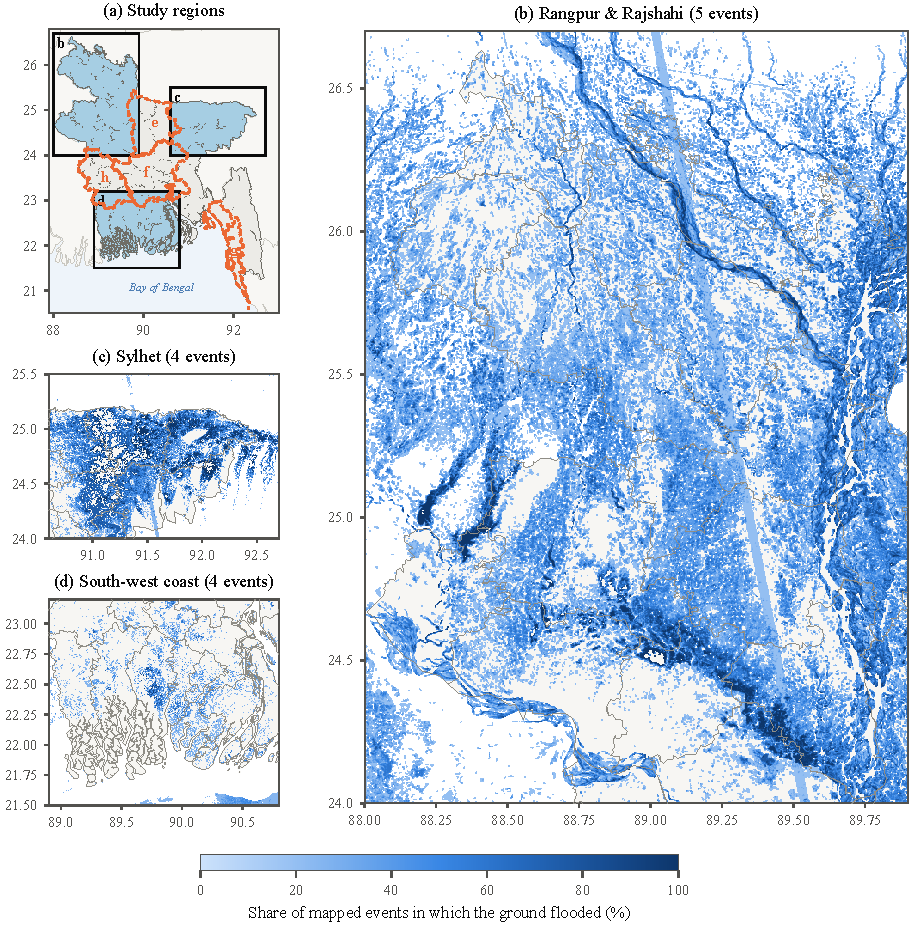
\includegraphics[width=0.92\textwidth]{figures/fig_study_frequency.pdf}
\caption{(a) The three study regions, drawn as their configured bounding boxes, and the validation region east of the Jamuna (e, dashed), over the district boundaries of geoBoundaries, with neighbouring countries from Natural Earth. (b--d) Share of the mapped Sentinel-1 events in which each 100\,m cell was flooded. Cells never seen flooded are left blank, and the removal of permanent water leaves the main river channels empty. Straight-edged bands follow the edges of radar swaths.}
\label{fig:study}
\end{figure*}

\begin{table*}[tp]
\centering
\small
\begin{tabular}{llll}
\toprule
Region & Hazard & Bounding box (W, S, E, N) & Configuration \\
\midrule
Rangpur \& Rajshahi & riverine flood & 88.0, 24.0, 89.9, 26.7 & \fileref{config.yaml} \\
Sylhet & flash flood & 90.6, 24.0, 92.7, 25.5 & \fileref{configs/sylhet.yaml} \\
South-west coast & coastal and tidal flooding & 88.9, 21.5, 90.8, 23.2 & \fileref{configs/sw\_coastal.yaml} \\
Jamuna east$^{a}$ & riverine and flash flood & 89.6, 23.9, 90.9, 25.5 & \fileref{configs/validation/jamuna\_east.yaml} \\
Central$^{a}$ & riverine flood & 89.25, 22.8, 91.08, 24.39 & \fileref{configs/validation/central.yaml} \\
Chattogram coast$^{a}$ & flash flood and surge & 91.26, 20.54, 92.4, 23.04 & \fileref{configs/validation/chattogram\_coast.yaml} \\
West-central$^{a}$ & waterlogging & 88.51, 22.75, 89.86, 24.24 & \fileref{configs/validation/west\_central.yaml} \\
\bottomrule
\end{tabular}
\caption{Configured study regions. $^{a}$Validation region, defined by its districts within the box and without any asset a study box holds. Each box is restricted to Bangladesh, and all use UTM zone 46N (EPSG:32646) for distance and area calculations.}
\label{tab:regions}
\end{table*}

\begin{table*}[tp]
\centering
\small
\begin{tabularx}{\textwidth}{lXll}
\toprule
Dataset & Use & Resolution & Licence \\
\midrule
OpenStreetMap & infrastructure assets (roads, bridges, schools, hospitals, shelters, embankments, cropland) & vector & ODbL 1.0 \\
SRTM 1 arc-second & elevation, slope, topographic wetness, height above drainage, flow accumulation & 30\,m & public domain \\
JRC Global Surface Water & historical water occurrence, one proxy-label vote & 30\,m & free with attribution \\
JRC global river flood hazard maps v2.1.2 (GloFAS) & reference ranking for later floods & 3 arc-seconds (about 90\,m) & CC BY 4.0 \\
WorldPop constrained 2020 & population density for vulnerability and population exposure & 100\,m & CC BY 4.0 \\
geoBoundaries gbOpen & districts (ADM2), upazilas (ADM3), unions (ADM4) & vector & CC BY 4.0 \\
Sentinel-1 GRD (via Earth Engine) & observed flood extents for training labels and validation & 10\,m, exported at 100\,m & Copernicus open \\
\bottomrule
\end{tabularx}
\caption{Datasets ingested by the pipeline. JRC is the European Commission Joint Research Centre and GloFAS its Global Flood Awareness System. National files (WorldPop, geoBoundaries, JRC tiles) are downloaded once into a shared cache and clipped per region.}
\label{tab:data}
\end{table*}

\section{Methods}
\label{sec:chain}

The pipeline runs as a chain of steps (Fig.~\ref{fig:chain}), and this section follows it in order. Settings not given here are in the Supporting Information (Section~S1).

\begin{figure*}[tp]
\centering
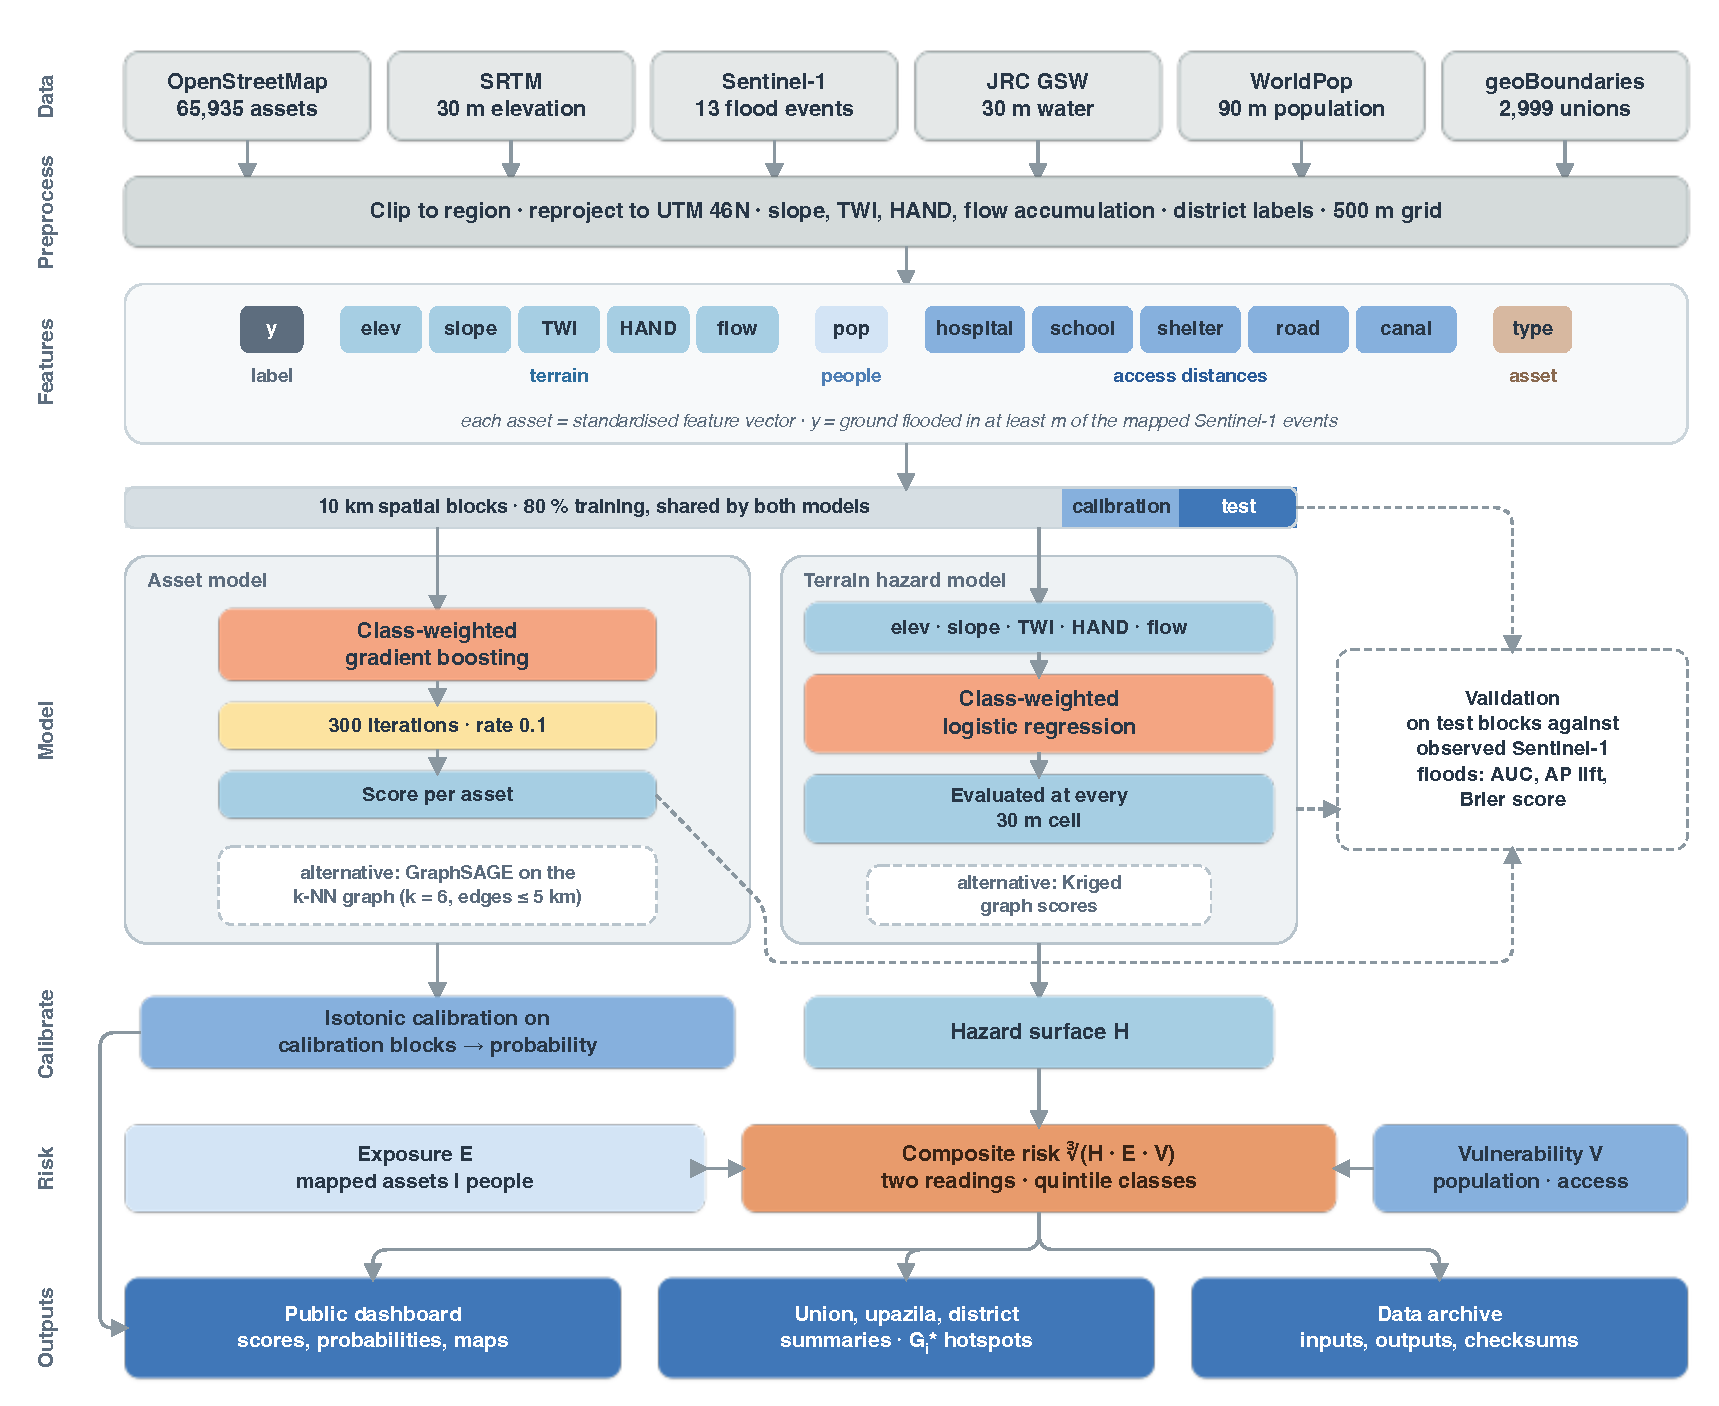
\includegraphics[width=\textwidth]{figures/fig_chain_flood.pdf}
\caption{The processing chain, top to bottom. Source counts are totals over the three flood regions. Each asset enters the models as a vector of terrain, population, access-distance and asset-type features, with a label from the Sentinel-1 flood frequency. The asset model is expanded, with the graph network it replaced shown as the alternative it now is. Both models train on the same spatial blocks, and dashed connectors mark what the validation scores on the test blocks.}
\label{fig:chain}
\end{figure*}

\subsection{Assets, terrain and features}

Assets are fetched from OpenStreetMap in three tag groups, lifelines (hospitals, schools, shelters, bridges, embankments), transport (primary to trunk roads, railways) and agriculture (farmland, aquaculture, canals, markets), and each is classified into one asset type. The configured boxes cross Bangladesh's land border, so assets in India, or on land more than about 1\,km outside the geoBoundaries border, are dropped, while those on chars, coastal ground and offshore are kept. Grid cells and grid-level validation are restricted the same way. From the 30\,m SRTM elevation model, reprojected to UTM zone 46N, the pipeline derives slope, the topographic wetness index (TWI), height above nearest drainage (HAND) and D8 flow accumulation. FABDEM, which removes forest and building heights \citep{hawker2022}, would suit a flat delta better, but its non-commercial, share-alike licence conflicts with the CC BY 4.0 data archive, and the vertical error of SRTM may be one reason, untested, why TWI and HAND add little once elevation is known (Section~\ref{sec:importance}). Each asset carries these five terrain values at its representative point, WorldPop population density, its distance to the nearest hospital, school, flood shelter, road and irrigation channel, and its asset type, all standardised, and the pipeline stops if any feature is constant or the labels hold a single class.

\subsection{Flood extents from Sentinel-1}
\label{sec:observed}

Flood extents mapped from Sentinel-1 radar supply both the training labels and the reference against which the models are scored. Following the change-detection method recommended by UN-SPIDER \citep{unspider}, an approach whose best Sentinel-1 variant reached an overall accuracy of 86.3\,\% against reference flood maps in an evaluation for Thailand \citep{dadhich2026}, the minimum VV backscatter in each flood window is compared in Google Earth Engine with the median of a dry-season baseline from the same year. A pixel is flagged as flooded where it is below $-16$\,dB and at least 3\,dB darker than its baseline. Permanent water from the JRC record \citep{pekel2016}, slopes above 5$^\circ$ and specks under eight pixels are removed, and the event masks are averaged into a flood-frequency layer (Fig.~\ref{fig:study}b--d). Five events are mapped in Rangpur and Rajshahi, four in Sylhet and four cyclone landfalls on the coast, each window set from ReliefWeb situation reports (Table~\ref{tab:events}).

The masks were checked against an independent map of two of the same floods, the August 2017 flood in Rangpur and Rajshahi and the April 2017 haor flood in Sylhet, which the Global Flood Database maps from MODIS at 250\,m \citep{tellman2021}. On that grid, over cells that MODIS saw clear and that are not permanent water, the maps agree on \RRXcAgree{}\,\% and \SylhetXcAgree{}\,\% of cells, a figure dominated by dry ground. On flooded ground the agreement is only moderate, with a critical success index of \RRXcCSI{} and \SylhetXcCSI{} and a kappa of \RRXcKappa{} and \SylhetXcKappa{}. The radar marks more ground as flooded than MODIS in Rangpur and Rajshahi (\RRXcSOneShare{}\,\% against \RRXcGfdShare{}\,\%), consistent with flooded patches smaller than a MODIS pixel and with flooding hidden by cloud. It marks less in the Sylhet haor (\SylhetXcSOneShare{}\,\% against \SylhetXcGfdShare{}\,\%), consistent with the difficulty radar has where water stands under vegetation \citep{amitrano2024}, as it did under unharvested rice in April 2017. Neither explanation was tested, and neither map is ground truth.

\begin{table*}[tp]
\centering
\small
\begin{tabularx}{\textwidth}{llX}
\toprule
Region & Window & Basis \\
\midrule
Rangpur \& Rajshahi & 12--26 Aug 2017 & second monsoon flood from 12 August; Dinajpur, Kurigram, Lalmonirhat and Rangpur among the worst affected \\
 & 12--26 Jul 2019 & rain from 9 July, Brahmaputra--Jamuna rising to 18 July, Kurigram more than 1\,m above danger level \\
 & 11--31 Jul 2020 & second phase from 9--10 July, peak about 18 July, 27 basin gauges above danger into late July \\
 & 28 Jun--16 Jul 2024 & northern floods from mid-June, Brahmaputra above danger at Nunkhawa, Hatia and Chilmari in early July \\
 & 27 Sep--12 Oct 2024 & Teesta flooding of Lalmonirhat, Nilphamari, Kurigram and Rangpur from late September \\
\midrule
Sylhet & 30 Mar--20 Apr 2017 & haor flooding from 28 March, striking Sunamganj on 1 April \\
 & 15--26 Jun 2022 & heavy rain from 15 June, situation worst from 17 June \\
 & 16--28 Jun 2024 & 2.25 million affected in Sylhet, Sunamganj and Moulvibazar by 22 June \\
 & 18--30 Aug 2024 & eastern floods from 20 August, including Moulvibazar and Habiganj \\
\midrule
South-west coast & 20--31 May 2020 & Cyclone Amphan, landfall 20 May \\
 & 25 May--4 Jun 2021 & Cyclone Yaas, landfall 26 May \\
 & 23 Oct--2 Nov 2022 & Cyclone Sitrang, landfall 24--25 October \\
 & 26 May--5 Jun 2024 & Cyclone Remal, landfall 26--27 May \\
Jamuna east & 12--26 Aug 2017 & second monsoon flood from 12 August \\
 & 13--28 Jul 2019 & Brahmaputra--Jamuna rising to 18 July \\
 & 11--31 Jul 2020 & second phase from 9--10 July, peak about 18 July \\
 & 3--15 Oct 2024 & north-central flash floods from 3 October in Sherpur, Mymensingh and Jamalpur; first Sentinel-1 pass on 8 October \\
Central & 15--31 Aug 2017 & Faridpur, Rajbari, Manikganj and Munshiganj among the affected districts \\
 & 18 Jul--2 Aug 2019 & monsoon flood reaching the central districts by 19 July \\
 & 15 Jul--10 Aug 2020 & second phase of the 2020 monsoon flood \\
Chattogram coast & 5--15 Aug 2023 & flash floods and monsoon rain in Chattogram division \\
 & 26 May--1 Jun 2024 & Cyclone Remal \\
 & 20 Aug--5 Sep 2024 & eastern flash floods \\
West-central & 13--30 Sep 2024 & waterlogging of low-lying Jessore after heavy rain \\
 & 25 Jul--25 Aug 2025 & waterlogging of the Bhabodah area \\
\bottomrule
\end{tabularx}
\caption{Flood events mapped from Sentinel-1. Windows bracket the flood peak; the baseline for each is the February--March dry season of the same year (mid-January to March for the pre-monsoon haor event). Sources are ReliefWeb and United Nations situation reports and, for the west-central waterlogging, national newspapers, all cited in the configuration files.}
\label{tab:events}
\end{table*}

\subsection{Training labels}
\label{sec:labels}

In the riverine regions ground counts as flood-prone where it flooded in at least two of the mapped events, while on the coast one cyclone window is enough, because surge drains within days and the six-to-twelve-day revisit leaves too few pixels flooded twice. The pipeline also writes a terrain-threshold ensemble, which marks a pixel as flood-prone where at least two of three indicators agree, TWI above 8, HAND below 5\,m and JRC water occurrence above 25\,\%. TWI and HAND are also model inputs, so a model trained and scored on these labels can succeed by relearning the threshold rule.

\subsection{Asset model}
\label{sec:gnn}

The default asset model is class-weighted gradient boosting with 300 iterations and a learning rate of 0.1, which matched or beat a random forest, logistic regression and a two-layer GraphSAGE network \citep{hamilton2017} on a six-nearest-neighbour graph of assets, the design this system began with (Supporting Information, Section~S7). Validation holds out whole 10\,km blocks, assigned at random to training (80\,\%), calibration and test, because a random split leaves every test asset beside training assets with almost the same features and label. Scores are calibrated by isotonic regression on the calibration blocks, with each level shrunk towards the middle when it holds few points, and every metric comes from the test blocks. In the two riverine regions the published map scores come from the same model given one more feature, the share of earlier events in which the ground flooded (Section~\ref{sec:temporal}). Every validation figure outside that section comes from the model without it, because the feature is built from the events the models are scored against.

\subsection{Validation design}
\label{sec:design}

Every model is scored on the held-out blocks by the area under the ROC curve (AUC), average precision and its lift over the base rate, and the Brier score. Every comparison between models or label sources is repeated over \RRBenchSeeds{} block assignments drawn with different seeds. The paired differences are tested by the corrected resampled t-test of \citet{nadeau2003}, since the assignments reuse the same assets, and a plain t-test across them would overstate the evidence. The 10\,km blocks are narrower than the ranges of the variograms fitted to the asset scores, roughly \RRVariogramRangeKm{}, \SylhetVariogramRangeKm{} and \CoastalVariogramRangeKm{}\,km, so test assets near a block edge still share terrain with training assets, and the main results are repeated with 20 and 40\,km blocks on the same seeds (Section~\ref{sec:blocksize}).

\subsection{Later floods and published maps}
\label{sec:rolling}

The model and the record are compared on later floods in two designs. The first trains on the floods up to 2022 and scores against those of 2024 (Section~\ref{sec:temporal}). The second, a rolling origin, makes every flood year with an earlier event a test in turn. The model learns from the earlier years only, under the region's labelling rule capped by their number of events, the record is the share of those events in which the ground flooded, and both are scored on the held-out blocks against that year's floods. Each test also records the share of that year's flooded assets standing on ground no earlier flood had reached, termed new ground here, the quantity expected to decide which of the two ranks better. Four validation regions join the three study regions in this design, the Jamuna east bank, the central districts around Dhaka, the Chattogram coast and the west-central districts, each a region of a national partition of Bangladesh with every asset that a study box also holds removed, matched by OpenStreetMap identity or by location (Table~\ref{tab:regions}). Distances there run to every facility of the region, including those removed.

Two published maps are scored on the same assets. The JRC global river flood hazard maps \citep{baugh2024}, simulated with LISFLOOD-FP at about 90\,m for return periods of 10 to 500 years, give each asset the annual exceedance probability of the most frequent flood that reaches it. JRC Global Surface Water occurrence \citep{pekel2016}, the share of Landsat observations from 1984 to 2021 that saw water, stands for a record available anywhere without processing radar and is scored only against floods after 2021. Besides AUC, every ranking is scored by its Molchan trajectory and area skill score \citep{zechar2008}, with every asset weighted equally, so that a random ranking scores 0.5, and by the prediction accuracy index \citep{chainey2008} of a list as long as the record's, the share of flooded assets the list holds divided by the share of assets it flags.

\section{Results}
\label{sec:validation}

\subsection{Held-out results}

Table~\ref{tab:validation} reports one block assignment, the pipeline's default, which ranks \RRDefaultSeedRank{}, \SylhetDefaultSeedRank{} and \CoastalDefaultSeedRank{} of \RRBenchSeeds{} by AUC in the three regions. In Sylhet \SylhetLabelRate{}\,\% of assets sit on flood-prone ground and the asset model reaches an AUC of \SylhetValAUC{}. In Rangpur and Rajshahi only \RRLabelRate{}\,\% do, yet the model ranks well (AUC \RRValAUC{}), with an average precision \RRValAPLift{} times the base rate. Calibration lowers the Brier score from \RRValBrier{} to \RRValBrierCalibrated{} in Rangpur and Rajshahi, slightly below the \RRValBrierBaseRate{} of always predicting the base rate, and its deciles lie close to the diagonal in both riverine regions (Fig.~\ref{fig:calibration}). It carries less well to the coast, where the calibration blocks hold \CoastalCalibBlockRate{}\,\% flood-prone assets against \CoastalTestBlockRate{}\,\% in the test blocks and the calibrated Brier score of \CoastalValBrierCalibrated{} is worse than the base rate at \CoastalValBrierBaseRate{}.

\begin{table*}[tp]
\centering
\small
\begin{tabular}{lrrrrrr}
\toprule
Region & Assets & Positive rate & Asset AUC & Asset AP & Brier & Terrain AUC \\
\midrule
Rangpur \& Rajshahi & \RRAssets{} & \RRLabelRate{}\,\% & \RRValAUC{} & \RRValAP{} & \RRValBrier{} & \RRHazardAUC{} \\
Sylhet & \SylhetAssets{} & \SylhetLabelRate{}\,\% & \SylhetValAUC{} & \SylhetValAP{} & \SylhetValBrier{} & \SylhetHazardAUC{} \\
South-west coast & \CoastalAssets{} & \CoastalLabelRate{}\,\% & \CoastalValAUC{} & \CoastalValAP{} & \CoastalValBrier{} & \CoastalHazardAUC{} \\
\bottomrule
\end{tabular}
\caption{Validation on held-out 10\,km test blocks, for the pipeline's default block assignment, from the model without the past-flooding feature that the riverine maps carry (Section~\ref{sec:gnn}). Positive rate is the share of assets on ground the radar saw flood in the required number of events. The Brier score is that of the raw class-weighted scores, and the calibrated probabilities are reported in the text. Means over repeated assignments, lower in the riverine regions and higher on the coast, are in the Supporting Information, Table~S3.}
\label{tab:validation}
\end{table*}

\subsection{Observed extents against terrain labels}
\label{sec:labelresult}

The terrain-threshold ensemble captures \RRProxyPOD{} of the ground that flooded in at least \RRMinEvents{} of the five Rangpur and Rajshahi events, with a false alarm ratio of \RRProxyFAR{}, and marks \RRProxyShare{}\,\% of the region as flood-prone where the radar saw \RRObservedShare{}\,\% flood that often. Trained on those labels and scored on the same held-out blocks against observed flooding over \RRBenchSeeds{} assignments, the default model reaches \RRLabelProxyAUC{} against \RRLabelObsAUC{} for observed labels in Rangpur and Rajshahi, \SylhetLabelProxyAUC{} against \SylhetLabelObsAUC{} in Sylhet and \CoastalLabelProxyAUC{} against \CoastalLabelObsAUC{} on the coast. The gaps of \RRLabelGap{}, \SylhetLabelGap{} and \CoastalLabelGap{} favour the observed labels on \RRLabelAhead{}, \SylhetLabelAhead{} and \CoastalLabelAhead{} of the assignments (\AllLabelGapP{}; Fig.~\ref{fig:roc}). This test favours the observed labels, since that model is scored against the definition it learned, so Section~\ref{sec:temporal} repeats it against later floods that neither label source was trained on.

\begin{figure*}[tp]
\centering
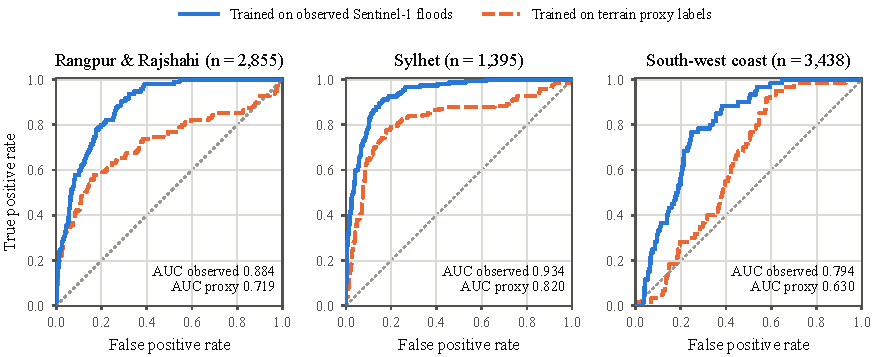
\includegraphics[width=\textwidth]{figures/fig_roc.pdf}
\caption{ROC curves on the held-out test blocks of each flood region, scored against the observed definition of flood-prone ground. Both curves come from the default gradient-boosted model on one block assignment, sharing features and blocks and differing only in their training labels. The dotted diagonal is a random ranking, and $n$ is the number of assets in the test blocks.}
\label{fig:roc}
\end{figure*}

\begin{figure*}[tp]
\centering
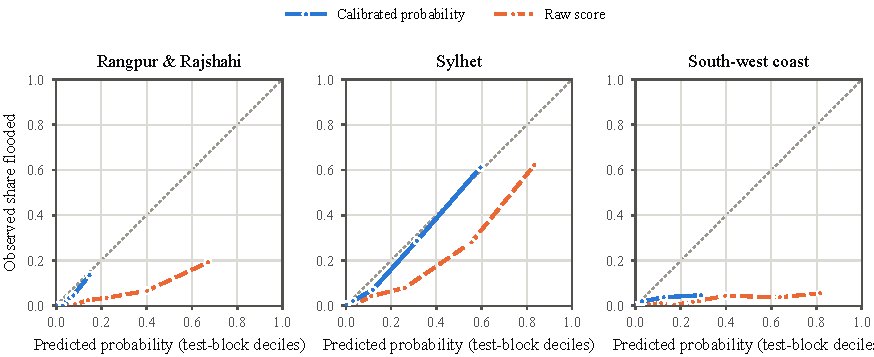
\includegraphics[width=\textwidth]{figures/fig_calibration.pdf}
\caption{Reliability of the flood model on the test blocks, with assets grouped into deciles of each prediction. The raw class-weighted score overstates the likelihood of flooding. The isotonic calibration, fitted on other blocks, brings the riverine deciles close to the diagonal. On the coast, where the calibration blocks hold more flood-prone ground than the test blocks (\CoastalCalibBlockRate{}\,\% against \CoastalTestBlockRate{}\,\%), it still overstates the flooding observed.}
\label{fig:calibration}
\end{figure*}

\subsection{Transfer to later floods}
\label{sec:temporal}

The held-out blocks separate training from testing in space but not in time. Each model is therefore also trained on the floods up to 2022, keeping each region's labelling rule capped by the number of earlier events, and scored on the held-out blocks against the ground any 2024 flood reached. Three references are scored on the same assets over \RRTempSeeds{} assignments (Table~\ref{tab:temporal}). The first is the share of earlier events in which the ground flooded, which is the map the radar record alone provides. The second is the same model trained with the 2024 events included, and the third is the same model trained on terrain-threshold labels, which draw on no flood event.

\begin{table*}[tp]
\centering
\small
\begin{tabular}{lcccc}
\toprule
Region & Model to 2022 & All events & Past flooding & Terrain labels \\
\midrule
Rangpur \& Rajshahi & \RRTempAUC{} $\pm$ \RRTempSD{} & \RRTempAllAUC{} & \RRTempPastAUC{} $\pm$ \RRTempPastSD{} & \RRTempProxyAUC{} $\pm$ \RRTempProxySD{} \\
Sylhet & \SylhetTempAUC{} $\pm$ \SylhetTempSD{} & \SylhetTempAllAUC{} & \SylhetTempPastAUC{} $\pm$ \SylhetTempPastSD{} & \SylhetTempProxyAUC{} $\pm$ \SylhetTempProxySD{} \\
South-west coast & \CoastalTempAUC{} $\pm$ \CoastalTempSD{} & \CoastalTempAllAUC{} & \CoastalTempPastAUC{} $\pm$ \CoastalTempPastSD{} & \CoastalTempProxyAUC{} $\pm$ \CoastalTempProxySD{} \\
Jamuna east (validation) & \JamunaTempAUC{} $\pm$ \JamunaTempSD{} & \JamunaTempAllAUC{} & \JamunaTempPastAUC{} $\pm$ \JamunaTempPastSD{} & \JamunaTempProxyAUC{} $\pm$ \JamunaTempProxySD{} \\
\bottomrule
\end{tabular}
\caption{AUC against the 2024 flood extents on held-out 10\,km test blocks, as mean $\pm$ standard deviation over \RRTempSeeds{} block assignments. The model to 2022 is trained only on the earlier events, the all-events model on labels that include 2024, past flooding is the share of the earlier events in which the ground flooded, and the terrain-label model is the same model trained on the terrain-threshold labels. The 2024 events reached \RRTempTestRate{}\,\%, \SylhetTempTestRate{}\,\%, \CoastalTempTestRate{}\,\% and \JamunaTempTestRate{}\,\% of assets in the four regions, and east of the Jamuna only \JamunaTempSeeds{} assignments left flooded assets in the test blocks.}
\label{tab:temporal}
\end{table*}

Trained only on earlier floods, the model ranks the 2024 flooding at \RRTempAUC{} in Rangpur and Rajshahi, \SylhetTempAUC{} in Sylhet and \CoastalTempAUC{} on the coast. In both riverine regions the record of earlier flooding ranks it better, at \RRTempPastAUC{} and \SylhetTempPastAUC{}, with the model ahead on only \RRTempAheadPast{} and \SylhetTempAheadPast{} of \RRTempSeeds{} assignments, whereas on the coast the model leads, at \CoastalTempAUC{} against \CoastalTempPastAUC{}. The regions differ in how often floods return to the same ground, since only \RRPastFeatUnseenPos{}\,\% and \SylhetPastFeatUnseenPos{}\,\% of the assets flooded in 2024 stood on ground no earlier event had reached, against \CoastalPastFeatUnseenPos{}\,\% on the coast, where each surge floods the stretch of coast where it lands. The 2024 floods in Rangpur and Rajshahi were also small, covering \RRLateExtentMin{}--\RRLateExtentMax{}\,\% of the region against \RREarlyExtentMin{}--\RREarlyExtentMax{}\,\% for each earlier flood, whereas in Sylhet they were as large as earlier ones.

Seven checks test whether the comparison favours one side (Supporting Information, Section~S5, Table~S1), and in Rangpur and Rajshahi the record keeps its lead under all of them, if narrowly under two. Re-mapped from Sentinel-1A alone, since Sentinel-1B failed in December 2021 and fewer scenes can map less flooding, the earlier events shrank by up to \RRSingleSatShrinkMax{}\,\% and the record still led by \RRSingleSatGap{}. Retrained on flooding in any earlier event, which is how the 2024 floods are counted, the model fell further behind, by \RRTargetAnyGap{}, and with 40\,km blocks the lead grew to \RRBlockFortyTempGap{}. In Sylhet the record's lead closed, to \SylhetTargetAnyGap{}, when the model learned the same target as the test, so the Sylhet result rests on the choice of target, and on the coast the model's lead fell within noise with 20 and 40\,km blocks.

East of the Jamuna, where the October 2024 flood reached only \JamunaPlanAllFlooded{} assets, the record again led, at \JamunaTempPastAUC{} against \JamunaTempAUC{} on held-out blocks, but with a handful of flooded assets in most test blocks the lead fell short of significance ($p\JamunaTempMinusPastP{}$) except with 40\,km blocks ($p\JamunaBlockFortyTempP{}$). Out of fold over the whole region it led at \JamunaOofRecordAUC{} against \JamunaOofModelAUC{}, with a block-bootstrap interval for the difference from \JamunaOofGapLow{} to \JamunaOofGapHigh{}, and its list of \JamunaPlanListShare{}\,\% of assets held \JamunaPlanAllRecord{}\,\% of the flooded assets against \JamunaPlanAllModel{}\,\% for the model.

The record can also enter the model as a feature, provided it comes from floods before the ones the model learns to predict, or the model would copy its own labels. The model is therefore trained to predict the last event year up to 2022 from its usual features and the share of the earlier events in which the ground flooded, and scored against the 2024 floods with that share taken over every event to 2022. In Rangpur and Rajshahi the combination beats both of its parts, at \RRPastFeatAUC{} against \RRPastFeatOnlyAUC{} for the record alone ($p\RRPastFeatOverPastP{}$) and \RRPastFeatWithoutAUC{} for the model without the feature. Its gain comes on the ground no earlier flood reached, \RRPastFeatUnseenShare{}\,\% of the test assets, where the record gives every asset a score of zero and the combined model still ranks the 2024 flooding at \RRPastFeatUnseenAUC{}. In Sylhet the combination, at \SylhetPastFeatAUC{}, cannot be told apart from the model without the feature ($p\SylhetPastFeatOverWithoutP{}$) or the record alone ($p\SylhetPastFeatOverPastP{}$). On the coast, where the design leaves a single cyclone to train on, the combination at \CoastalPastFeatAUC{} cannot be told apart from the record alone ($p\CoastalPastFeatOverPastP{}$).

Measured as skill over the record (Supporting Information, Section~S6), the share of the record's remaining ranking error that a model removes, the model scored \RRSkillModel{} in Rangpur and Rajshahi, \SylhetSkillModel{} in Sylhet and \CoastalSkillModel{} on the coast, and \RRSkillPastFeat{} in Rangpur and Rajshahi given the record as a feature. A list of every asset an earlier flood reached held \RRPlanAllRecord{}\,\% of the assets the 2024 floods reached in Rangpur and Rajshahi against \RRPlanAllModel{}\,\% for an equally long list from the model. On the coast, where the model ranked better overall, the record's list of \CoastalPlanListShare{}\,\% of assets still held \CoastalPlanAllRecord{}\,\% against \CoastalPlanAllModel{}\,\%, marking the most exposed ground more precisely even where it ranked the rest worse.

The 2024 floods also give the label comparison a test that favours neither label source. The observed labels still lead, at \RRTempAUC{} against \RRTempProxyAUC{} in Rangpur and Rajshahi, \SylhetTempAUC{} against \SylhetTempProxyAUC{} in Sylhet and \CoastalTempAUC{} against \CoastalTempProxyAUC{} on the coast, ahead on \RRTempProxyAhead{}, \SylhetTempProxyAhead{} and \CoastalTempProxyAhead{} of \RRTempSeeds{} assignments. The coastal gap of \CoastalTempProxyGap{} stays close to its spatial \CoastalLabelGap{}, while the riverine gaps shrink, from \RRLabelGap{} to \RRTempProxyGap{} in Rangpur and Rajshahi and from \SylhetLabelGap{} to \SylhetTempProxyGap{} in Sylhet, where the remaining gap cannot be told apart from noise. Much of the Sylhet advantage in the spatial test therefore came from the shared definition rather than from the labels themselves.

\subsection{Every flood year}
\label{sec:rollresult}

Predicting every flood year from the years before it gives \PoolTests{} tests, \PoolStudyTests{} in the study regions and \PoolValidationTests{} in the validation regions (Table~\ref{tab:rolling}). The record ranked the later flooding significantly better in \PoolRecordWins{}, the model in \PoolModelWins{}, and in the other \PoolTies{} the two could not be told apart, so the 2024 result in Rangpur and Rajshahi is not the rule for every year. The share of new ground decided which way a test went, ranging from \PoolNewGroundMin{} to \PoolNewGroundMax{}\,\% (Fig.~\ref{fig:lead}a). The record's lead fell as that share rose (Spearman $\rho=\PoolRho{}$, $p\PoolRhoP{}$), in the study regions ($\rho=\PoolStudyRho{}$) and the validation regions ($\rho=\PoolValidationRho{}$, $p\PoolValidationRhoP{}$) alike, and the fitted line crosses zero at \PoolCrossing{}\,\% (95\,\% interval \PoolCrossingLow{}--\PoolCrossingHigh{}\,\%). New ground shrinks as the record lengthens, but the relation held with the number of earlier years held fixed (partial $\rho=\PoolPartialRho{}$, $p\PoolPartialP{}$), while that number added nothing once new ground was known ($\rho=\PoolYearsPartialRho{}$). The relation also held with each region left out in turn and within every region with more than one test, although resampling whole regions widened the crossover interval to \RegionBootCrossingLow{}--\RegionBootCrossingHigh{}\,\% (Section~S9). In Rangpur and Rajshahi the model ranked the 2019 flood better, when \RRRollNineteenNewGround{}\,\% of it reached new ground, the two were level in 2020, and the record led in 2024, at \RRRollTwentyFourNewGround{}\,\%. Given the record as a feature, the model ranked the later flooding above both of its parts in \CombinedAheadBoth{} of \CombinedTests{} tests, all riverine.

The JRC hazard map ranked the later floods at \MapAUCMin{} to \MapAUCMax{}, below chance on the coast, whose surges it does not simulate, so it is a fair rival only for river flooding. It trailed the record significantly in \MapRecordAheadSig{} tests and led it in \MapAheadSig{}, each on a flood that reached much new ground, and the model ranked above it in \MapModelAhead{} of \MapTests{}. Landsat water occurrence, scored on the \OccTests{} floods after 2021, ranked them at \OccAUCMin{} to \OccAUCMax{}, below the radar record in \OccBelowRecord{}. Area skill scores ordered the record and the model as AUC did in \AssAgree{} of \AssTests{} tests, and the Molchan trajectories show where the difference lay (Fig.~\ref{fig:lead}b, c). In Rangpur and Rajshahi the record caught most of the 2024 flooding within the first sixth of the assets it flagged and then, holding nothing on the rest, ran down the diagonal, while on the coast the model missed fewer flooded assets at most list lengths.

\begin{table*}[tp]
\centering
\footnotesize
\setlength{\tabcolsep}{4pt}
\begin{tabular}{llrrcccccc}
\toprule
 & & Earlier & New & & & Model & Hazard & Water & \\
Region & Year & years & ground (\%) & Record & Model & + record & map & occurrence & $p$ \\
\midrule
Rangpur \& Rajshahi & 2019 & \RRRollNineteenYears{} & \RRRollNineteenNewGround{} & \RRRollNineteenRecord{} & \RRRollNineteenModel{} & \RRRollNineteenBoth{} & \RRRollNineteenMap{} & \RRRollNineteenOcc{} & \RRRollNineteenPTab{} \\
Rangpur \& Rajshahi & 2020 & \RRRollTwentyYears{} & \RRRollTwentyNewGround{} & \RRRollTwentyRecord{} & \RRRollTwentyModel{} & \RRRollTwentyBoth{} & \RRRollTwentyMap{} & \RRRollTwentyOcc{} & \RRRollTwentyPTab{} \\
Rangpur \& Rajshahi & 2024 & \RRRollTwentyFourYears{} & \RRRollTwentyFourNewGround{} & \RRRollTwentyFourRecord{} & \RRRollTwentyFourModel{} & \RRRollTwentyFourBoth{} & \RRRollTwentyFourMap{} & \RRRollTwentyFourOcc{} & \RRRollTwentyFourPTab{} \\
Sylhet & 2022 & \SylhetRollTwentyTwoYears{} & \SylhetRollTwentyTwoNewGround{} & \SylhetRollTwentyTwoRecord{} & \SylhetRollTwentyTwoModel{} & \SylhetRollTwentyTwoBoth{} & \SylhetRollTwentyTwoMap{} & \SylhetRollTwentyTwoOcc{} & \SylhetRollTwentyTwoPTab{} \\
Sylhet & 2024 & \SylhetRollTwentyFourYears{} & \SylhetRollTwentyFourNewGround{} & \SylhetRollTwentyFourRecord{} & \SylhetRollTwentyFourModel{} & \SylhetRollTwentyFourBoth{} & \SylhetRollTwentyFourMap{} & \SylhetRollTwentyFourOcc{} & \SylhetRollTwentyFourPTab{} \\
South-west coast & 2021 & \CoastalRollTwentyOneYears{} & \CoastalRollTwentyOneNewGround{} & \CoastalRollTwentyOneRecord{} & \CoastalRollTwentyOneModel{} & \CoastalRollTwentyOneBoth{} & \CoastalRollTwentyOneMap{} & \CoastalRollTwentyOneOcc{} & \CoastalRollTwentyOnePTab{} \\
South-west coast & 2022 & \CoastalRollTwentyTwoYears{} & \CoastalRollTwentyTwoNewGround{} & \CoastalRollTwentyTwoRecord{} & \CoastalRollTwentyTwoModel{} & \CoastalRollTwentyTwoBoth{} & \CoastalRollTwentyTwoMap{} & \CoastalRollTwentyTwoOcc{} & \CoastalRollTwentyTwoPTab{} \\
South-west coast & 2024 & \CoastalRollTwentyFourYears{} & \CoastalRollTwentyFourNewGround{} & \CoastalRollTwentyFourRecord{} & \CoastalRollTwentyFourModel{} & \CoastalRollTwentyFourBoth{} & \CoastalRollTwentyFourMap{} & \CoastalRollTwentyFourOcc{} & \CoastalRollTwentyFourPTab{} \\
Jamuna east$^{a}$ & 2019 & \JamunaRollNineteenYears{} & \JamunaRollNineteenNewGround{} & \JamunaRollNineteenRecord{} & \JamunaRollNineteenModel{} & \JamunaRollNineteenBoth{} & \JamunaRollNineteenMap{} & \JamunaRollNineteenOcc{} & \JamunaRollNineteenPTab{} \\
Jamuna east$^{a}$ & 2020 & \JamunaRollTwentyYears{} & \JamunaRollTwentyNewGround{} & \JamunaRollTwentyRecord{} & \JamunaRollTwentyModel{} & \JamunaRollTwentyBoth{} & \JamunaRollTwentyMap{} & \JamunaRollTwentyOcc{} & \JamunaRollTwentyPTab{} \\
Jamuna east$^{a}$ & 2024 & \JamunaRollTwentyFourYears{} & \JamunaRollTwentyFourNewGround{} & \JamunaRollTwentyFourRecord{} & \JamunaRollTwentyFourModel{} & \JamunaRollTwentyFourBoth{} & \JamunaRollTwentyFourMap{} & \JamunaRollTwentyFourOcc{} & \JamunaRollTwentyFourPTab{} \\
Central$^{a}$ & 2019 & \CentralRollNineteenYears{} & \CentralRollNineteenNewGround{} & \CentralRollNineteenRecord{} & \CentralRollNineteenModel{} & \CentralRollNineteenBoth{} & \CentralRollNineteenMap{} & \CentralRollNineteenOcc{} & \CentralRollNineteenPTab{} \\
Central$^{a}$ & 2020 & \CentralRollTwentyYears{} & \CentralRollTwentyNewGround{} & \CentralRollTwentyRecord{} & \CentralRollTwentyModel{} & \CentralRollTwentyBoth{} & \CentralRollTwentyMap{} & \CentralRollTwentyOcc{} & \CentralRollTwentyPTab{} \\
Chattogram coast$^{a}$ & 2024 & \ChattogramRollTwentyFourYears{} & \ChattogramRollTwentyFourNewGround{} & \ChattogramRollTwentyFourRecord{} & \ChattogramRollTwentyFourModel{} & \ChattogramRollTwentyFourBoth{} & \ChattogramRollTwentyFourMap{} & \ChattogramRollTwentyFourOcc{} & \ChattogramRollTwentyFourPTab{} \\
West-central$^{a}$ & 2025 & \WestCentralRollTwentyFiveYears{} & \WestCentralRollTwentyFiveNewGround{} & \WestCentralRollTwentyFiveRecord{} & \WestCentralRollTwentyFiveModel{} & \WestCentralRollTwentyFiveBoth{} & \WestCentralRollTwentyFiveMap{} & \WestCentralRollTwentyFiveOcc{} & \WestCentralRollTwentyFivePTab{} \\
\bottomrule
\end{tabular}
\caption{Every flood year predicted from the years before it, as mean AUC on held-out 10\,km blocks over \RRBenchSeeds{} block assignments. New ground is the share of that year's flooded assets standing on ground no earlier flood had reached. The model given the record as a feature needs two earlier years, and the water occurrence ends in 2021, so it is scored only on later floods. The $p$-value is the corrected resampled t-test of model against record. $^{a}$Validation region.}
\label{tab:rolling}
\end{table*}

\begin{figure*}[tp]
\centering
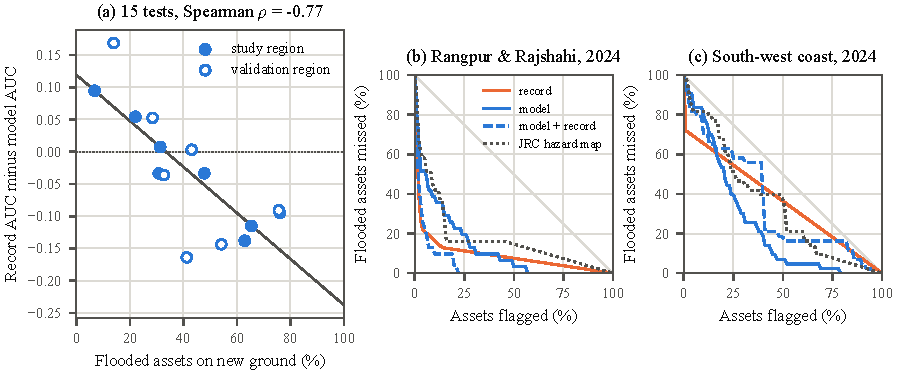
\includegraphics[width=\textwidth]{figures/fig_record_lead.pdf}
\caption{(a) The record's lead over the model in AUC against the share of each later flood that reached new ground, for every test in Table~\ref{tab:rolling}, with the least-squares line. (b, c) Molchan trajectories of the 2024 tests on one block assignment, the share of flooded assets missed against the share of assets flagged, lower being better; the grey diagonal is a random ranking.}
\label{fig:lead}
\end{figure*}

\subsection{Larger blocks}
\label{sec:blocksize}

Wider blocks lower the held-out AUC of the default model only a little in the riverine regions, from \RRLabelObsAUC{} at 10\,km to \RRBlockFortySpatialAUC{} at 40\,km in Rangpur and Rajshahi and from \SylhetLabelObsAUC{} to \SylhetBlockFortySpatialAUC{} in Sylhet, and more on the coast, from \CoastalLabelObsAUC{} to \CoastalBlockFortySpatialAUC{}, so the 10\,km figures carry a small optimism, largest on the coast.

\subsection{What the model relies on}
\label{sec:importance}

Shuffling each feature across the test assets over the same assignments shows what the default model uses (Fig.~\ref{fig:importance}). Elevation carries almost all of the terrain signal, costing \RRImpElevation{}, \SylhetImpElevation{} and \CoastalImpElevation{} in AUC when shuffled, while TWI, HAND, slope and flow accumulation cost at most \RRImpOtherTerrainMax{}, \SylhetImpOtherTerrainMax{} and \CoastalImpOtherTerrainMax{}. Shuffled together, since correlated features can stand in for one another, the five terrain features cost \RRImpTerrain{}, \SylhetImpTerrain{} and \CoastalImpTerrain{}, about as much as elevation alone, and slightly less in Rangpur and Rajshahi, a difference within the noise of the shuffling. The five access distances together cost \RRImpAccess{}, \SylhetImpAccess{} and \CoastalImpAccess{}, more than the terrain in Rangpur and Rajshahi and on the coast and second to it in Sylhet. They describe distance to services rather than any property of flooding and most likely stand in for where roads and settlements sit on the floodplain, a reading that was not tested directly.

\begin{figure*}[tp]
\centering
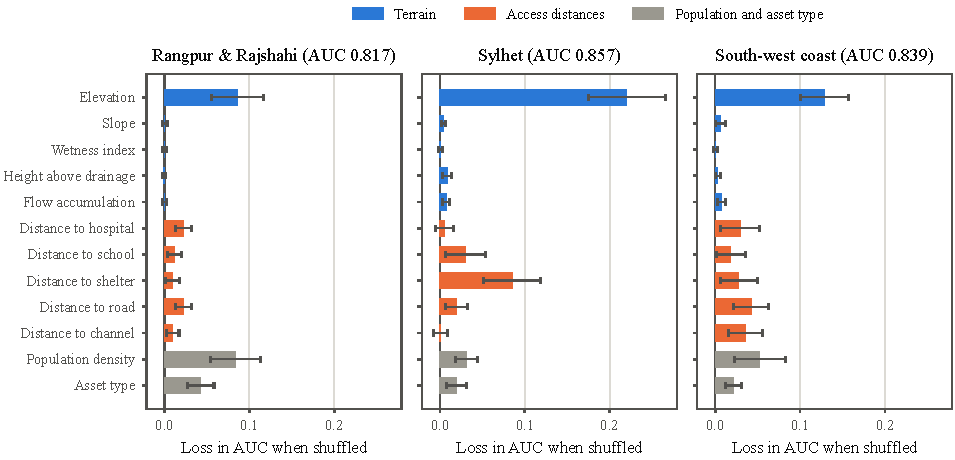
\includegraphics[width=\textwidth]{figures/fig_importance.pdf}
\caption{Loss in AUC on the held-out test blocks when each feature is shuffled across the test assets, as mean and standard deviation over \RRBenchSeeds{} block assignments, for the default gradient-boosted model. The AUC in each title is the mean before shuffling.}
\label{fig:importance}
\end{figure*}

\section{Discussion}
\label{sec:discussion}

\subsection{What the flood record already knows}

Whether a susceptibility model anticipates a later flood better than the record of earlier ones depended, across \PoolTests{} tests in seven regions, on how much of that flood reached new ground. Where less than about a third did, as in Rangpur and Rajshahi and Sylhet in 2024 and east of the Jamuna, the record ranked better or could not be told apart from the model, and where more did, as on the coast and in the first years of each record, the model ranked better in all but one test, significantly in \PoolModelWins{}. The share of new ground is known only after a flood, but in the riverine regions it fell as the record lengthened, from \RRRollNineteenNewGround{} to \RRRollTwentyFourNewGround{}\,\% in Rangpur and Rajshahi and from \JamunaRollNineteenNewGround{} to \JamunaRollTwentyFourNewGround{}\,\% east of the Jamuna, while on the coast, where each surge strikes its own stretch, it stayed near \CoastalRollTwentyFourNewGround{}\,\%. It is therefore a property of the flood regime that a record of a few events already reveals rather than an accident of one year. Earthquake forecasting reached the same verdict for a hazard that also recurs where it struck before, with neither a pattern-recognition model nor a national hazard map gaining on past seismicity \citep{zechar2008}, and the hydrodynamic map scored here, which trailed the record significantly in \MapRecordAheadSig{} tests, shows that the comparison bears on hazard maps generally and not only on machine learning. A published multi-criteria map of Sylhet scored on the same 2024 floods reached 0.794 \citep{swarup2026}, close to this model's \SylhetTempAUC{}, while the record ranked them at \SylhetTempPastAUC{}, a comparison that is only indicative, since that map was scored over areas.

The record marks where water returns and the terrain ranks where it has not yet been seen, and where floods recur the two combine well, the model given the record as a feature beating both in \CombinedAheadBoth{} of \CombinedTests{} tests. Floods returning to the same ground are expected on a floodplain, yet in Rangpur and Rajshahi a model scoring \RRBenchBoostingAUC{} on held-out blocks still ranked the 2024 flood below that expectation, at a skill over the record of \RRSkillModel{}. Forecasts are scored against persistence in the same way \citep{murphy1988, pappenberger2015}, and a susceptibility study that reports accuracy without that reference cannot show that its model knows more than the flood record already does.

\subsection{Labels decide what an accuracy figure means}

The label source decides what a published accuracy figure measures, since terrain-threshold labels cost the model \RRLabelGap{}, \SylhetLabelGap{} and \CoastalLabelGap{} in AUC on held-out blocks. The indices those labels are built on, TWI and HAND, add almost nothing to the model once elevation is known, and a model scored against labels derived from its own inputs measures its recovery of the labelling rule rather than its skill at locating floods. The mean AUCs here, \RRBenchBoostingAUC{} and \SylhetBenchBoostingAUC{} in the riverine regions, sit at or below the best-model AUCs of 0.87 to 0.98 in Table~\ref{tab:litflood}. The comparison is only indicative, since all but one of those studies split their points at random while every figure here comes from 10\,km blocks the model never saw. Blocking has its own critics \citep{roberts2017, wadoux2021}, and the blocked scores estimate performance on unseen areas of similar terrain rather than design-based map accuracy.

\subsection{Implications for flood risk management}
\label{sec:implications}

First, where Sentinel-1 has observed several floods, the record of where water has already stood is a benchmark any susceptibility map should beat, and where floods return to the same ground it was the better guide to the next one. It costs little to compute, so agencies such as the Bangladesh Water Development Board and the Flood Forecasting and Warning Centre could publish it as a planning layer beside any susceptibility map. Where the record holds only one or two flood years, or where surges strike new stretches of coast, the model ranked better, and the two combined ranked best on the riverine floodplains, so the choice between them can follow how much of past floods fell on new ground. Second, a susceptibility map used to site shelters, embankments or schools should be judged on held-out areas and later floods rather than on random splits, since the accuracy a random split reports overstates how far the map can be trusted in places it has not seen.

\subsection{Limits of the maps}

The coast is the clearest limit, since the terrain hazard surface reaches only \CoastalHazardHeldoutAUC{} there on held-out ground and the river hazard map ranks surge flooding below chance, because surge follows embankments, tidal channels and landfall position, which neither describes. The composite risk index (Supporting Information, Section~S2) depends on OpenStreetMap, whose rural completeness is unmeasured, and has not been checked against losses. The radar labels carry error of their own, agreeing only moderately with an independent MODIS map and counting inundated paddy as flooding, so every score here measures agreement with flooding mapped by radar rather than with flooding on the ground. Each test draws on one to three earlier flood years, and the threshold near a third of flooding on new ground is estimated from \PoolTests{} tests in \PoolRegions{} regions, with an interval of \PoolCrossingLow{} to \PoolCrossingHigh{}\,\% when tests are resampled and \RegionBootCrossingLow{} to \RegionBootCrossingHigh{}\,\% when whole regions are. The calibrated probabilities hold for a region as a whole rather than for any one area, and none of the surfaces is a forecast.

\section{Conclusions}
\label{sec:conclusions}

A flood susceptibility model knew more than the flood record only where floods reached new ground. Across \PoolTests{} tests in seven regions of Bangladesh, the record's lead over a terrain model fell as the share of each flood reaching new ground rose ($\rho=\PoolRho{}$), and the two were level at about \PoolCrossing{}\,\% of flooded assets. In Rangpur and Rajshahi the record predicted the 2024 flooding better than the model under every check applied, a global hydrodynamic hazard map was no stronger a rival, and a model given the record as a feature beat both of its parts in most riverine tests. Radar-observed flood extents made better training labels than terrain thresholds, by \RRLabelGap{}, \SylhetLabelGap{} and \CoastalLabelGap{} in AUC on held-out ground and by \RRTempProxyGap{}, \SylhetTempProxyGap{} and \CoastalTempProxyGap{} against later floods. Every number in this paper is generated from the released pipeline outputs, so each can be checked and rebuilt.

\section*{Data availability statement}

The data that support the findings of this study are openly available in Zenodo at \url{https://doi.org/10.5281/zenodo.23573843}. The code that produced them is openly available at \url{https://github.com/rakibhhridoy/rimes-mapathon} under the MIT licence. The repository holds the pipeline, region configurations, dashboard and test suite. The pipeline also holds a landslide susceptibility module for the Chittagong Hill Tracts, which is described in the technical documentation and will be reported separately. The Zenodo archive packages the input data and outputs for the three study regions, the four validation regions and the Hill Tracts, per region with a manifest of checksums and licences, together with the rolling-origin outputs. Every figure in this paper is written into the text by the analysis scripts in the code repository directly from the pipeline outputs, so a rerun of the pipeline updates text and results together. The results are published through an open dashboard at \url{https://fermium.systems/hazmapper}, which shows the risk maps, rankings and per-unit summaries without a sign-in and states the limitations of Section~\ref{sec:discussion} beside the maps. An earlier technical report on this system, prepared for the RIMES Mapathon in March 2026, contained errors that were found in a later review, the most serious being a coordinate-system error that left every training label at zero. Each error and its correction is listed in the technical documentation in the code repository, and no result of that report is used here.

\section*{Declarations}

\textbf{Competing interests.} Md Rakib Hasan is affiliated with Fermium Systems, which hosts the public dashboard described here. The software is released under the MIT licence and the data under the open licences listed in Table~\ref{tab:data}, and no result depends on a proprietary component.

\textbf{Author contributions.} Md Rakib Hasan is the sole author and carried out the conceptualisation, methodology, software, formal analysis, investigation, validation, data curation, visualisation and writing.

\textbf{Ethics approval and consent.} Not applicable. The study uses public datasets only and involves no human participants.

\section*{Acknowledgements}

The author received no specific funding for this work. Infrastructure data are \copyright{} OpenStreetMap contributors, under the Open Database Licence. Population data are from WorldPop, University of Southampton, CC BY 4.0. Administrative boundaries are from geoBoundaries, William \& Mary geoLab, CC BY 4.0. Neighbouring country outlines in Figure~\ref{fig:study} are from Natural Earth, in the public domain. Surface-water occurrence is from the Joint Research Centre of the European Commission \citep{pekel2016}. Elevation is from the NASA Shuttle Radar Topography Mission. Sentinel-1 data are from the Copernicus programme of the European Union. The system was first developed for the RIMES Mapathon, ResilienceAI track.

\bibliographystyle{apalike}
\bibliography{references}

\end{document}

